\chapter{Evaluation} \label{chapt: evaluation}
In this chapter we present results for the Mercury middleware and the MPI-IO hints extensions for collective I/O proposed in previous chapters. For Mercury we consider a high energy physics code.
This application is representative of a class of HPC analysis applications that are becoming more and more common in workloads of leadership class systems. Our goal is to demonstrate that through
user guided I/O prefetching even a non-optimized application can improve its I/O utilization (and thus performance) of the file system.
For our ROMIO improvements we consider a range of collective I/O benchmarks that include synthetic and real application kernels. We run every benchmark with the baseline collective I/O implementation
in ROMIO and discuss in detail all the ext2ph performance implications; then we enable our NVM based optimization and show how the same performance implications can be mitigated or completely
cancelled when taking the global parallel file system out of the ext2ph critical I/O path.

\section{I/O Prefetching in ROOT}
Our target real world application is written using `ROOT', an object-oriented framework widely adopted in the experimental high energy physics community to build software 
for data analysis. The application runs on the Mogon cluster at the data processing center of the University of Mainz (ZDV), in Germany. It analyzes particle data read from 
an input file structure using the `ROOT' format (structured file format).

\begin{figure*}[!htb]
  \centering
  \begin{subfigure}[t]{0.7\textwidth}
    \centering
    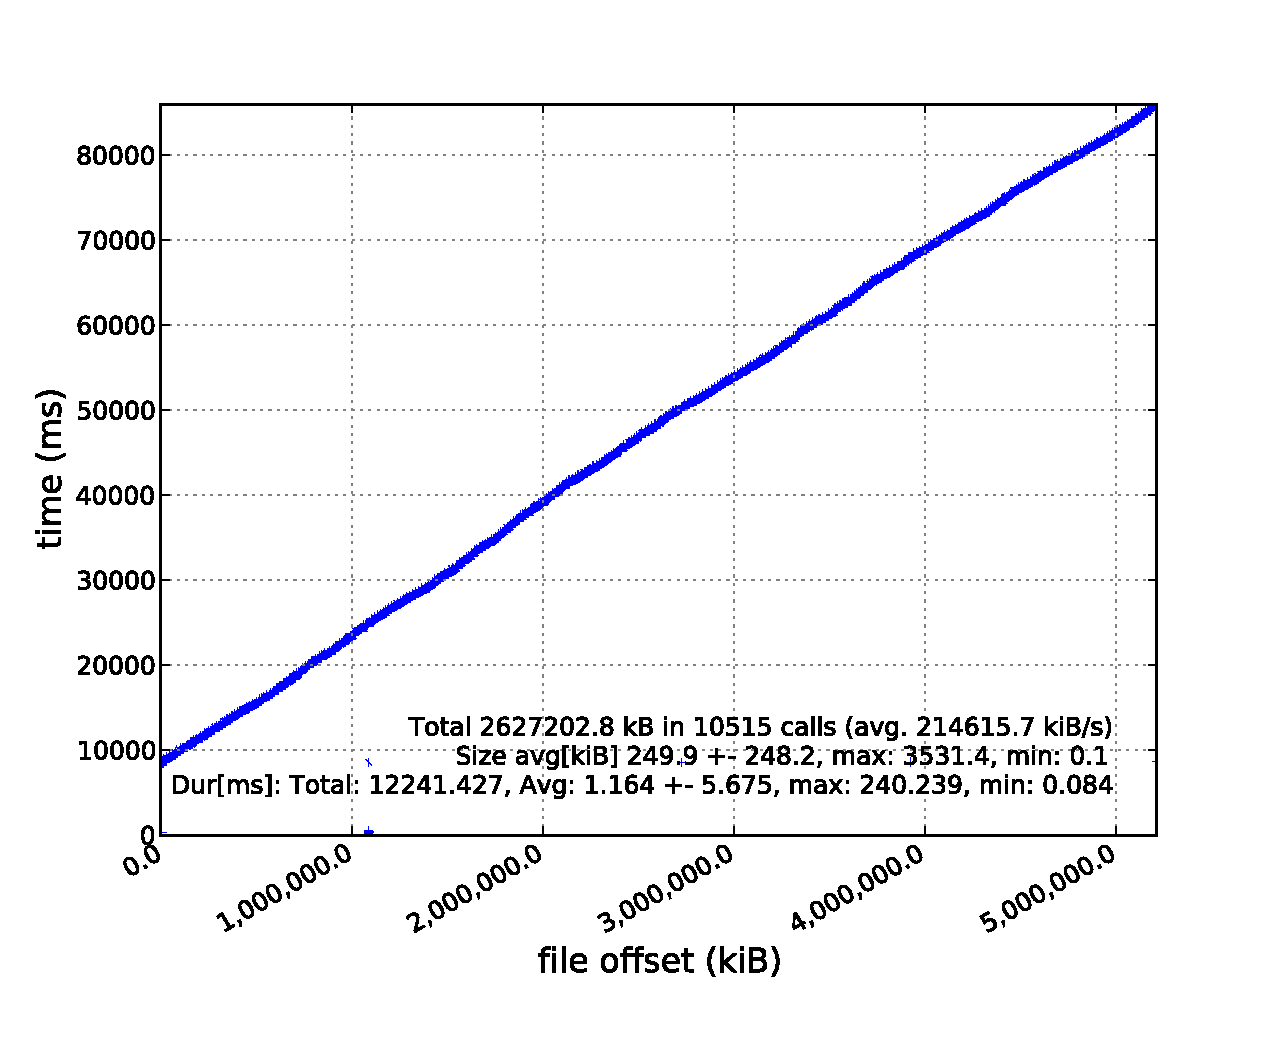
\includegraphics[width=\textwidth]{figures/iopat_profile}
    \caption{\textit{}}
    \label{figure: iopat_profile}
  \end{subfigure}
  \begin{subfigure}[t]{0.7\textwidth}
    \centering
    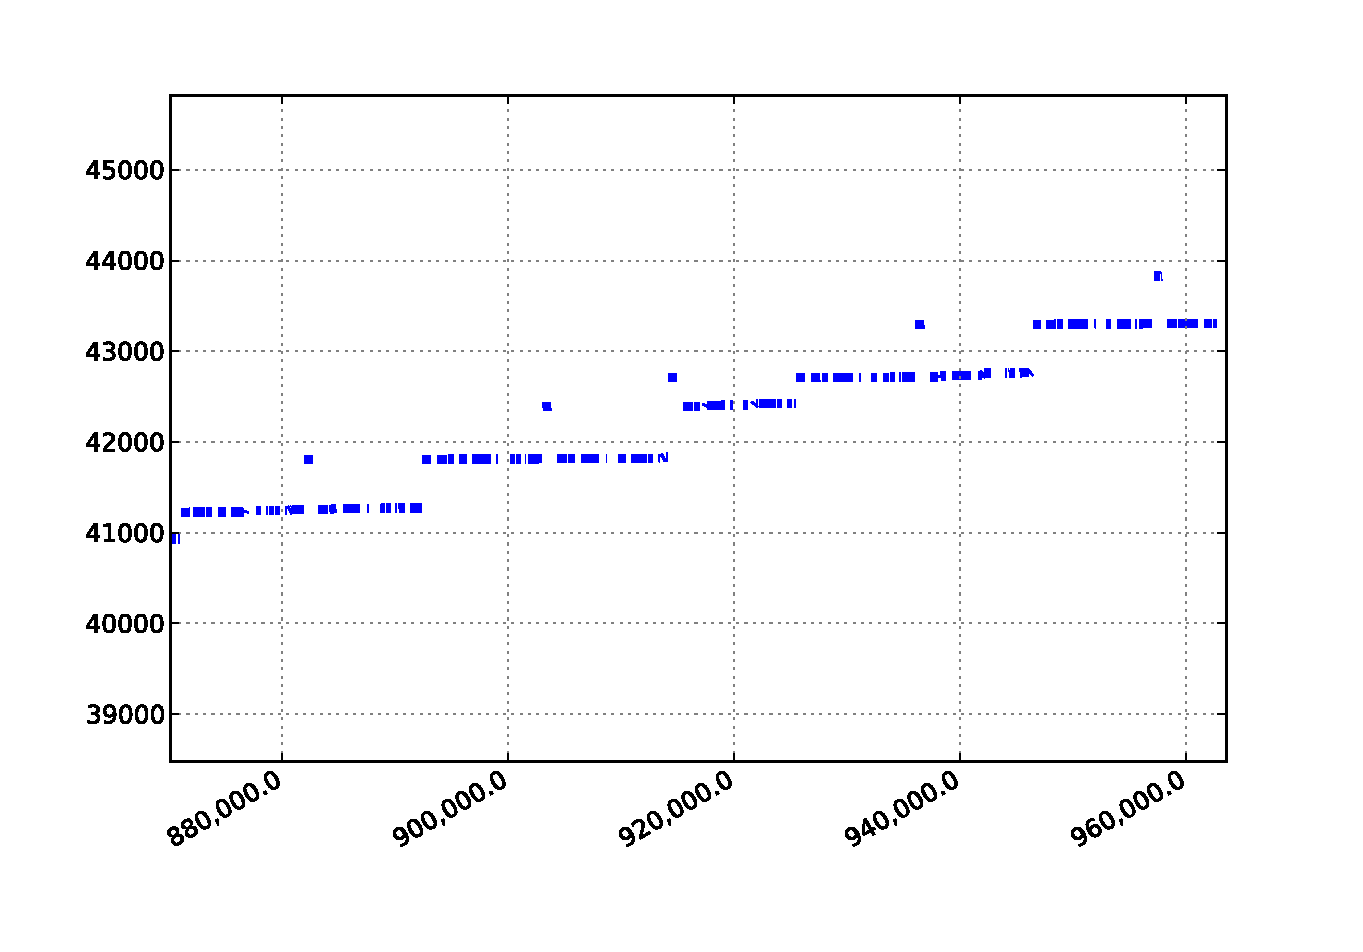
\includegraphics[width=\textwidth]{figures/00050_zoom}
    \caption{\textit{}}
    \label{figure: iopat_zoom}
  \end{subfigure}
  \caption{I/O read profile of the target application under analysis (\ref{figure: iopat_profile}), extracted from the the GPFS file system in the test cluster, and zoomed 
  window (\ref{figure: iopat_zoom}) showing the actual pattern details.}
  \label{figure: iopattern_with_statistics}
\end{figure*}

First of all we characterized the application's I/O pattern for a target file using traces and statistics extracted through several tools such as \textit{strace}, \textit{ioapps}\footnote{\url{https://code.google.com/p/ioapps}.} 
and GPFS's \textit{mmpmon} monitoring tool. 
Figure~\ref{figure: iopattern_with_statistics} shows the I/O pattern along with some additional statistics. As it can be seen, in this specific case (5 GB file), the application issues a total of 
10515 \texttt{read()} system calls to read about 2.6 GB of total data. The average request size is 250 KB and the time spent waiting for I/O is 12 seconds, when running on the test cluster. 

At a first glance the general I/O behaviour of the application looks sequential, most of the accesses to the file follow an increasing offset. Nevertheless, adjacent reads are separated by gaps 
(a strided read pattern). In a few cases this gap becomes negative, meaning that the application is moving backwards in the file to read some data previously left behind (as reported in 
Figure~\ref{figure: iopat_zoom}).

After a detailed I/O pattern analysis we could divide the target file into contiguous non-overlapping ranges. Within these ranges reads happen to have increasing offset. Even though the general 
I/O pattern of the application for different files looks similar\footnote{Due to space limits we do not report the comparison between different files.}, the size of the non-overlapping ranges may 
change significantly. This general behaviour can be modelled using Mercury through a configuration file in which a `WillNeed' hint covers the whole file from beginning to end (i.e., `Offset' and `Length' equal to 
0). The backwards seeks can be accounted for using the `CacheSize' parameter to keep previously accessed blocks in cache. In this way we effectively emulate a sliding window that tracks the application's 
I/O behaviour. This would not be possible by just using a, e.g., \texttt{POSIX\_FADV\_WILLNEED} advice on the whole file before starting the application like shown by Figure~\ref{figure: fadvise_comparison}. 
The reason is that if the file size is equal or smaller than the cache size, we would have a large number of valuable pages discarded from the cache to load data that will be accessed at the end of 
the application. Additionally, if the file size is bigger than the cache size we would have the file system discarding blocks at the beginning of the file as the blocks at the end are preloaded, 
effectively forcing the application to access these blocks from the I/O servers instead of the cache. With our approach, on the other hand, we keep in the cache only a small, controlled number of 
blocks (the ones currently accessed), while the older blocks are discarded since no longer needed. 

\begin{figure}[!htb]
  \centering
  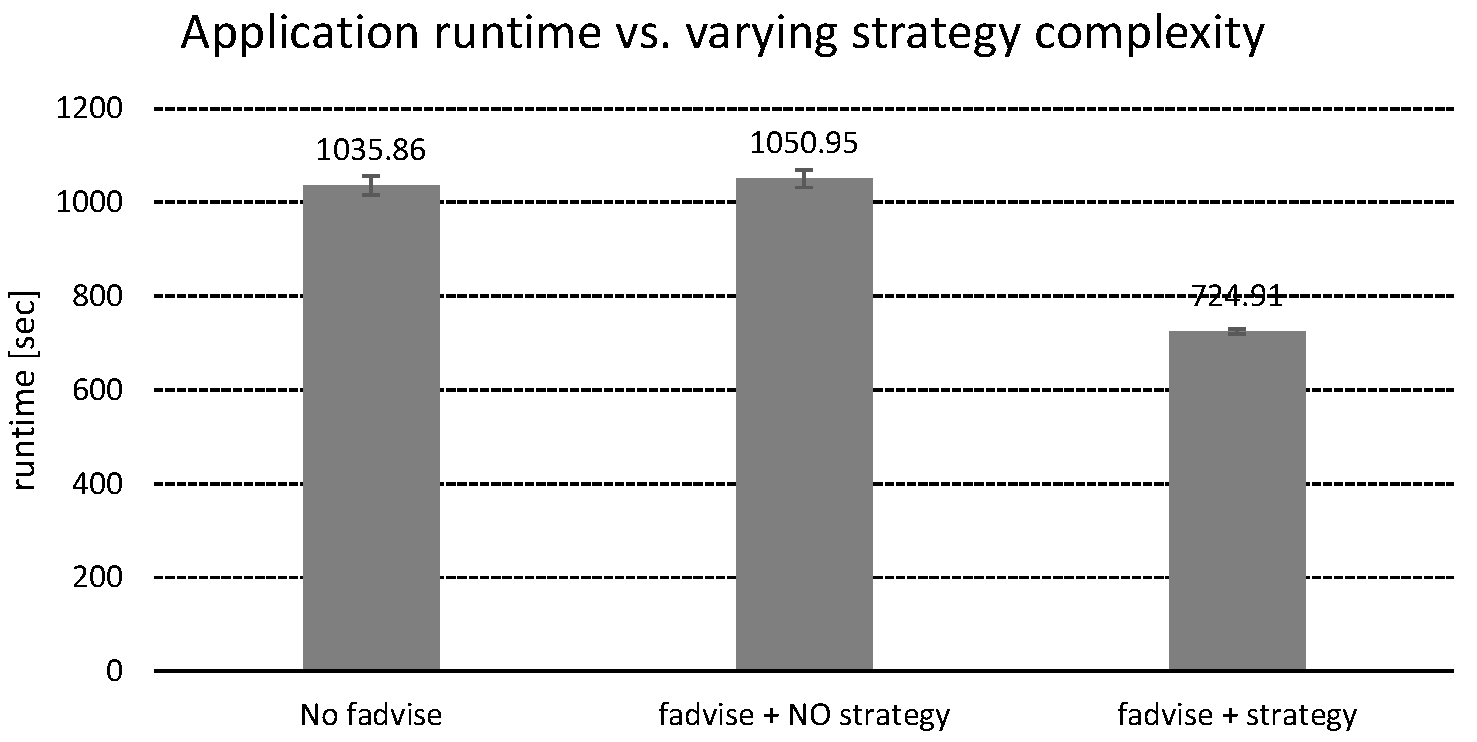
\includegraphics[width=0.8\textwidth]{figures/test_fadvise_no_border}
  \caption{Comparison between different usage stategies of posix\_fadvise for an input file of 55 GB residing in an ext4 file system. The first bar represents the case in which no advice is used, 
  the second bar represents the case in which a POSIX\_FADV\_WILLNEED is issued for the whole file at the beginning of the application and the third bar represents the case in which POSIX\_FADV\_WILLNEED 
  is issued using Mercury.}
  \label{figure: fadvise_comparison}
\end{figure} 

To assess the impact of our Mercury prototype on the application and file systems performance we considered the application execution time and the number of reads accounted for by the respective file systems. 
We conducted our experiments without file system hints and then with file system hints issued transparently to the application by the \textit{Advice Manager}. Furthermore, we ran each experiment three 
times and calculated average, minima and maxima for each metric. In order to avoid caching affecting our measurements, extra care was taken to clean all the relevant caches for the different file systems. 
For ext4 and Lustre this was accomplished by using the command line: $$echo\ 3 > /proc/sys/vm/drop\_caches$$ on the file system clients. Additionally, for Lustre this command was also executed on the
\textit{object storage servers} (OSSs) to avoid the server side cache to be retained. In the case of GPFS, the file system client's page pool was cleaned using the clean file cache hint in Table~\ref{table: hints_table}, 
the GPFS \textit{network shared disks} (NSDs)\footnote{GPFS name for I/O servers.} servers do not cache any data. 


\subsection{Test Bed}
Our testbed is composed by a test cluster of seven nodes, mainly intended to evaluate the proposed Linux kernel modifications with the Lustre file system. The reason 
for using a smaller cluster instead of the Mogon system is that it was not possible to disrupt the production cluster, affecting hundreds of users, by re-installing 
the operating system kernel. In order to make realistic comparisons between Lustre and GPFS, the test cluster also has a GPFS file system on comparable hardware. 

Both file systems have a single disk server each, one Dell R710 acts as GPFS network shared disk (NSD) server and another as Lustre object storage server. The R710 are equipped 
with two quadcore E5620 @2.4 GHz and 24 GB main memory. For storage, both disk servers share a MD3200 array with 2 controllers and 4 MD1200 expansion shelves for a total 
of 60 2 TB drives. The Storage is formatted in 4 15 dynamic disk pools. This is the LSI/Netapp type of declustered RAID, which distributes the 8+2 RAID6 stripes evenly 
over all 15 disks for better rebuild performance. The disk block size is set to 128 KB, which results in a RAID stripe size of 1 MB. The four disk pools are then split 
on the Array into LUNs, one of the LUNs from each disk pool is then used for GPFS and another one from each pool is used for Lustre. This results in comparable resources 
for both file systems and tests do not interfere with each other, as long as only one file system is tested at a time. 

While the GPFS filesystem embeds the metadata with the data, Lustre needs a separate Metadata Server (MDS). This is hosted by a SuperMicro server equipped with one quadcore Xeon 
E3-1230 @3.3 GHz and 16 GB of main memory, as metadata target (MDT) it uses a 120 GB SSD Intel 520. Four other machines of the same type, equipped with an eight core E3-1230 @3.3 
GHz processor and 16 GB of main memory, work as compute nodes and file system clients. All machines, servers and clients, are equipped with Intel X520DA 10 Gigabit adapters and 
connected to a SuperMicro SSE-X24S 24 ports 10 Gigabit switch. Both, the GPFS and Lustre file systems are formatted with a block size of 4 MB.

\subsection{Performance Results}
To measure the performance improvements that our Mercury prototype can deliver to the application's run-time we conducted two set of tests. In the first test we varied the size of the input file from 5 to 95 GB. 
This is mainly aimed to study the behaviour of the `ROOT' application using different input file sizes and how our solution behaves when the file becomes bigger than the available cache space. In the second 
test we varied the number of `ROOT' instances running simultaneously from 1 to 8. By doing so we study the interaction of multiple processes accessing the file system and how these can benefit from the prefetching 
hints generated by Mercury. Figures~\ref{figure: run-time_1} and~\ref{figure: run-time_2} report the results for the described experiments. All the tests where performed using a `BlockSize' of 4 MB, a `CacheSize' of 
8 blocks, a `ReadAheadSize' of 4 blocks, and a `WillNeed' hint covering the whole file (i.e., with `Offset' and `Length' equal to 0), resulting in each process consuming up to 32 MB of cache space and 512 MB in total 
for 8 application instances. 

The `WillNeed' on the whole file causes the \textit{Advisor Thread} to issue up to 4 (`ReadAheadSize') prefetching requests for blocks of 4 MB sequentially, starting from the current accessed 
block. This has the same effect of data sieving in ROMIO, optimizing the access size and allowing the application to read the requested data randomly from the cache instead of the file system. The produced effect is 
particularly beneficial in the case of Lustre and ext4, as it can be seen in Figures~\ref{figure: ext4_1} and~\ref{figure: lustre_1}. In these cases we measure reductions in the execution time of up to 50\%, with respect 
to the normal case. For GPFS we can still observe an improvement, but this is more contained compared to the other file systems (Figure~\ref{figure: gpfs_1}). The reductions in the execution time measured in GPFS are on 
average up to 10\%, with respect to the normal case. The reason is that the default prefetching strategy in GPFS works better that traditional read-ahead. In fact, by disabling the prefetching in GPFS we observed reductions 
in the execution time comparable to the other file systems (not reported here).

%\begin{figure}[!htb]
%  \centering
%  \begin{subfigure}[t]{0.48\textwidth}
%    \centering
%    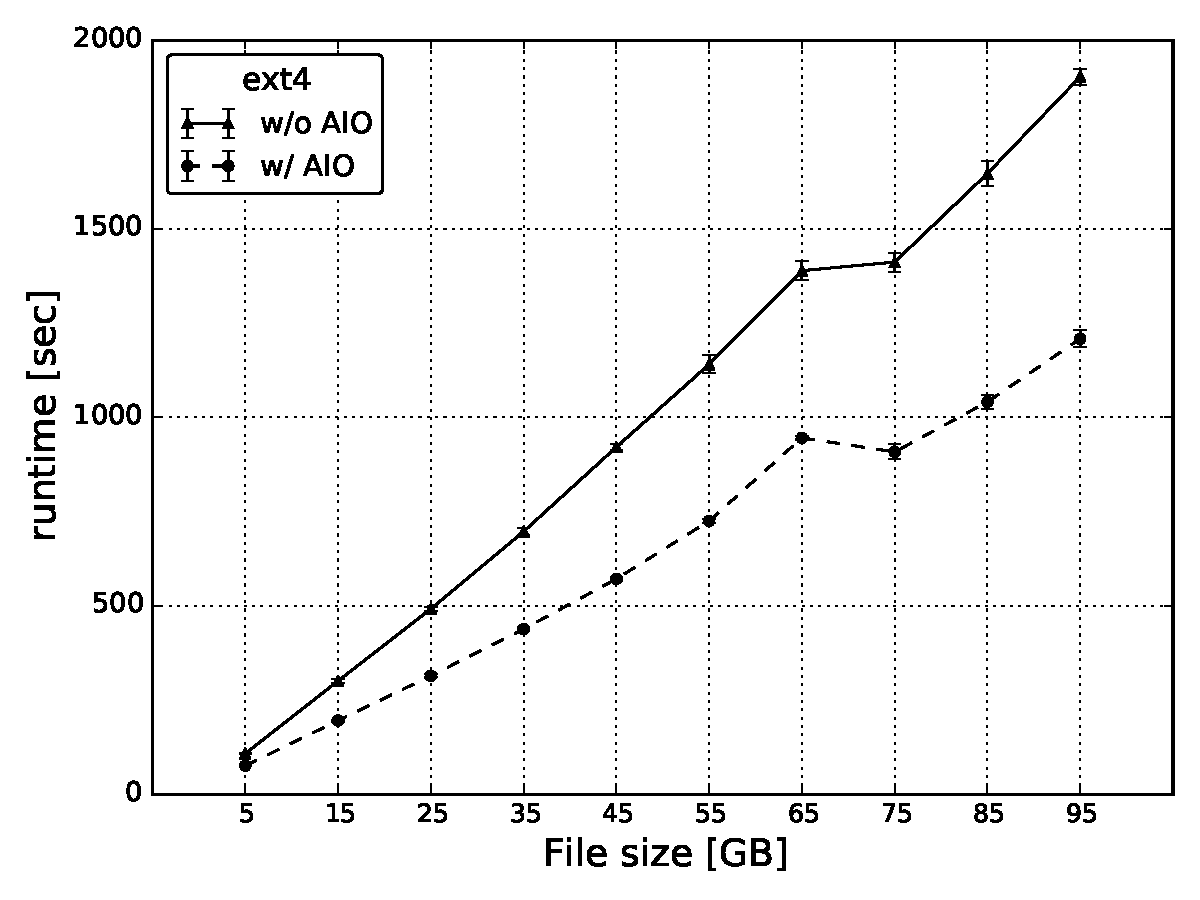
\includegraphics[width=\textwidth]{figures/ext4/runtime}
%    \caption{\textit{}}
%    \label{figure: ext4_1}
%  \end{subfigure}
%  \begin{subfigure}[t]{0.48\textwidth}
%    \centering
%    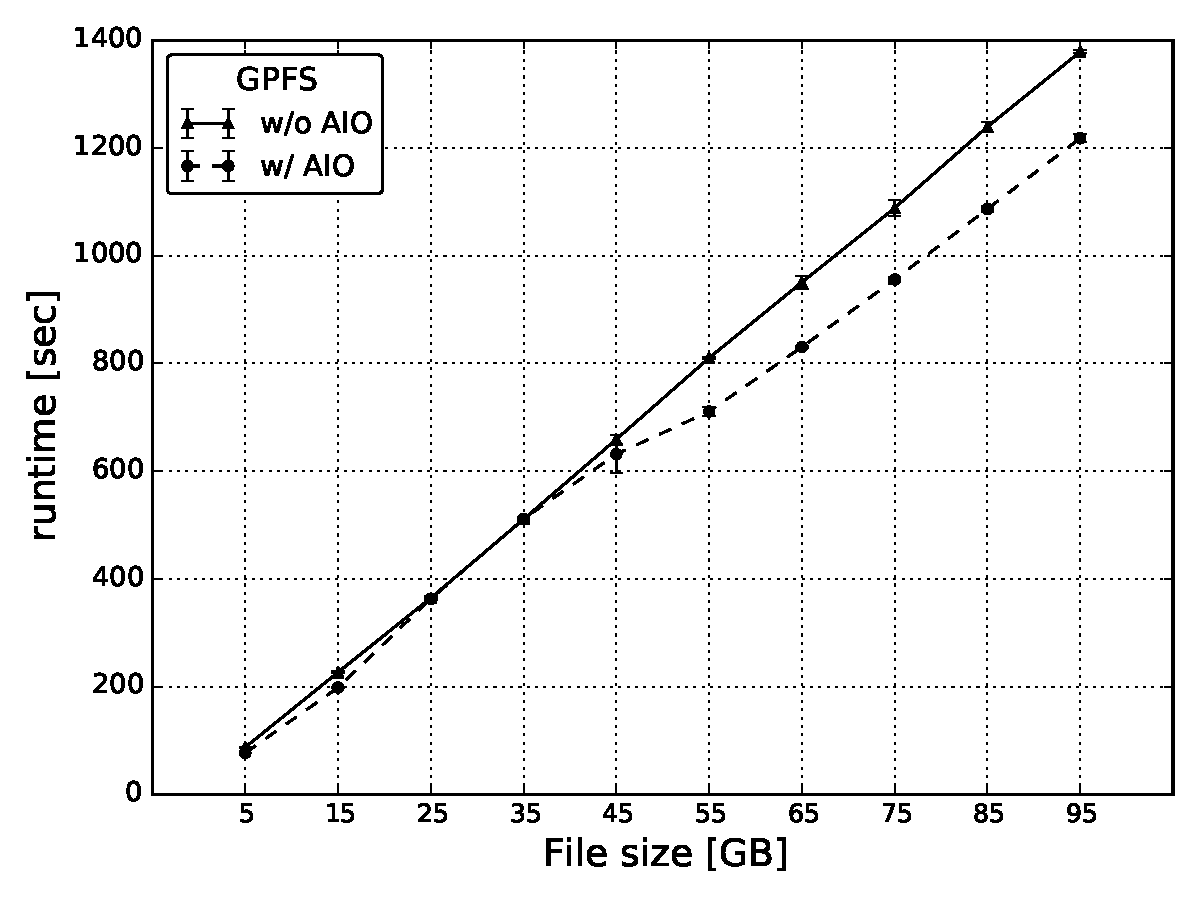
\includegraphics[width=\textwidth]{figures/gpfs/runtime}
%    \caption{\textit{}}
%    \label{figure: gpfs_1}
%  \end{subfigure}
%  \begin{subfigure}[t]{0.48\textwidth}
%    \centering
%    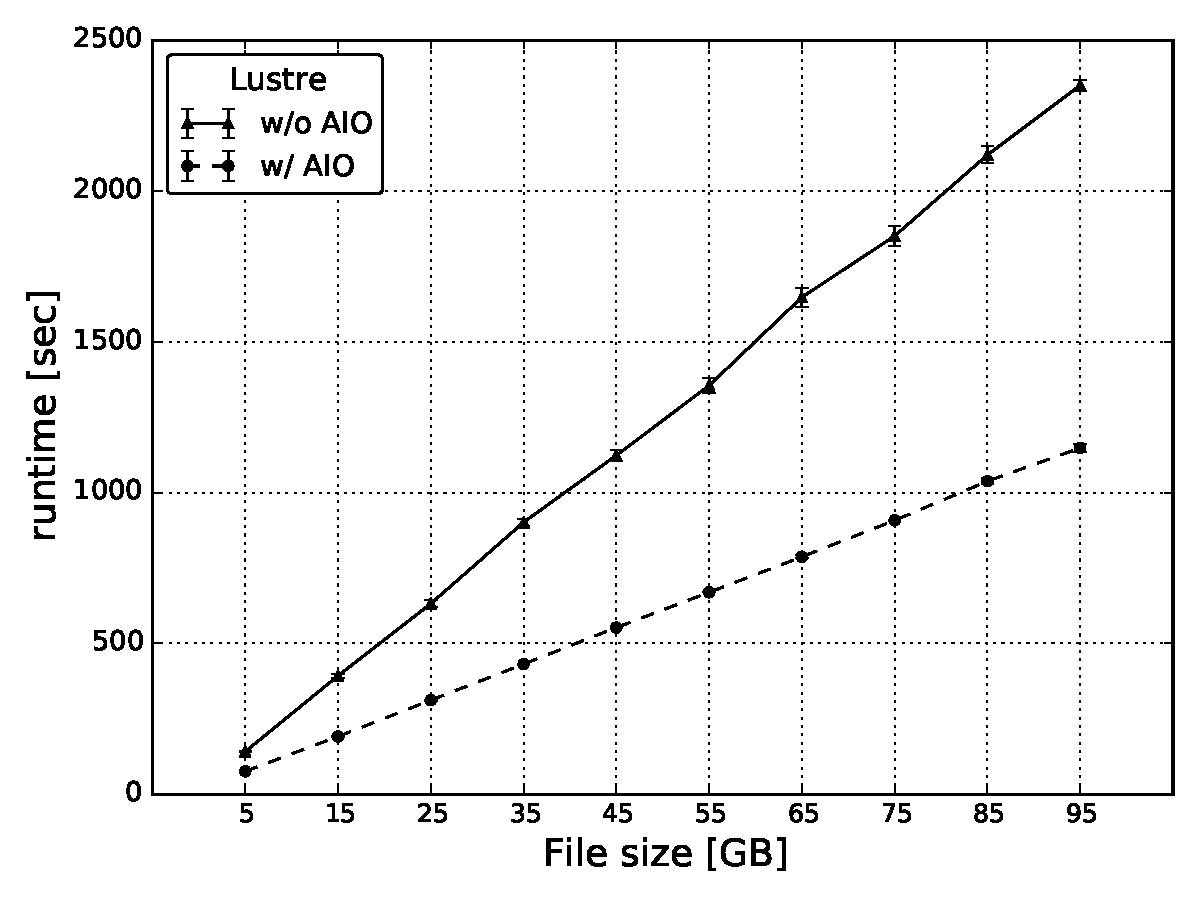
\includegraphics[width=\textwidth]{figures/Lustre/runtime}
%    \caption{\textit{}}
%    \label{figure: lustre_1}
%  \end{subfigure}
%  \caption{Running time of the ROOT application for the three file systems under study using different input file sized (\ref{figure: ext4_1},~\ref{figure: gpfs_1} and~\ref{figure: lustre_1}).}
%  \label{figure: run-time_1}
%\end{figure}
%
%\begin{figure}[!htb]
%  \centering
%  \begin{subfigure}[b]{0.48\textwidth}
%    \centering
%    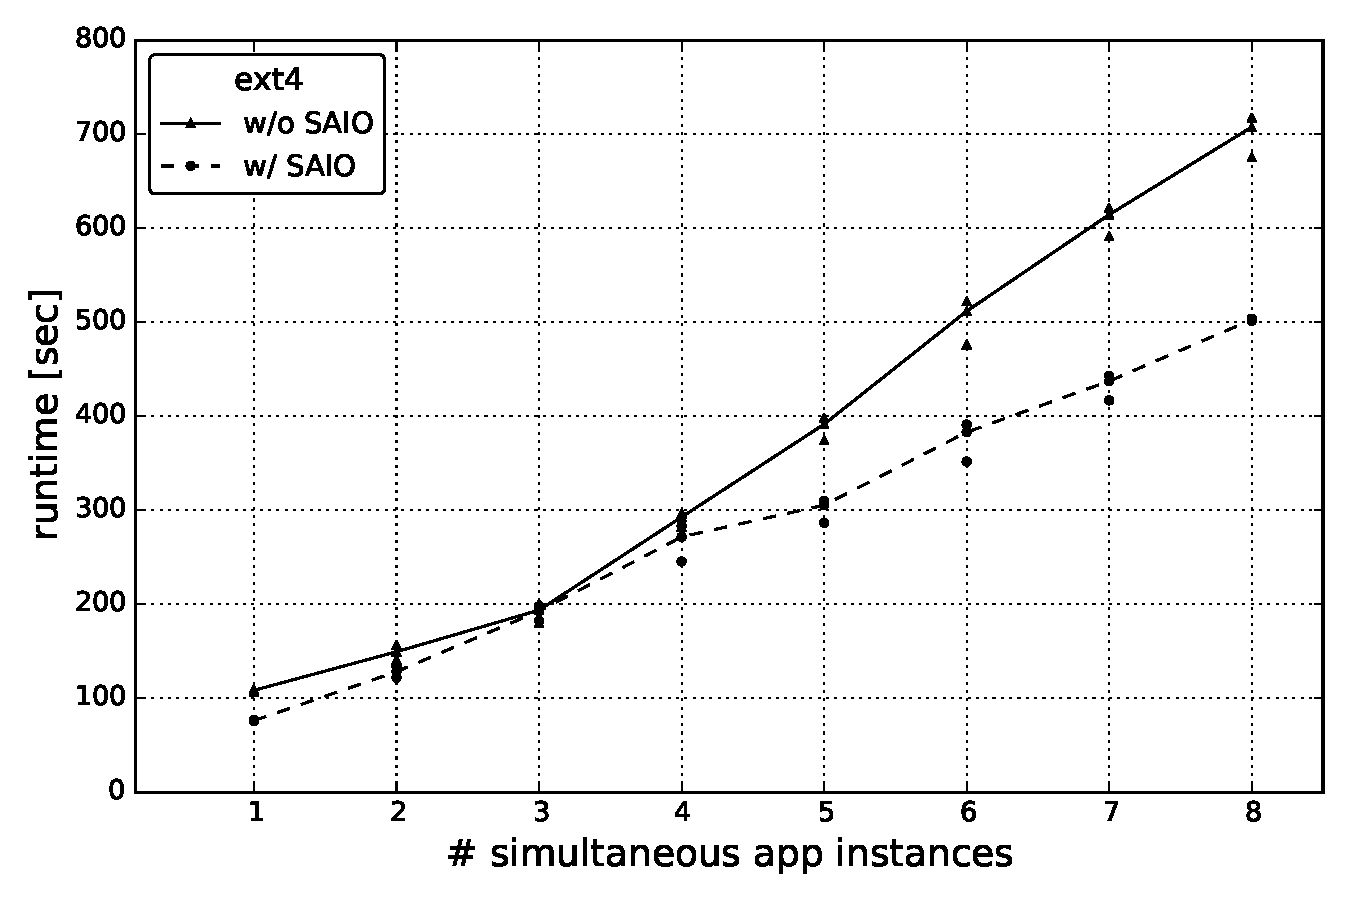
\includegraphics[width=\textwidth]{figures/simult_instance_ext4_test_cluster}
%    \caption{\textit{}}
%    \label{figure: ext4_2}
%  \end{subfigure}
%  \begin{subfigure}[b]{0.48\textwidth}
%    \centering
%    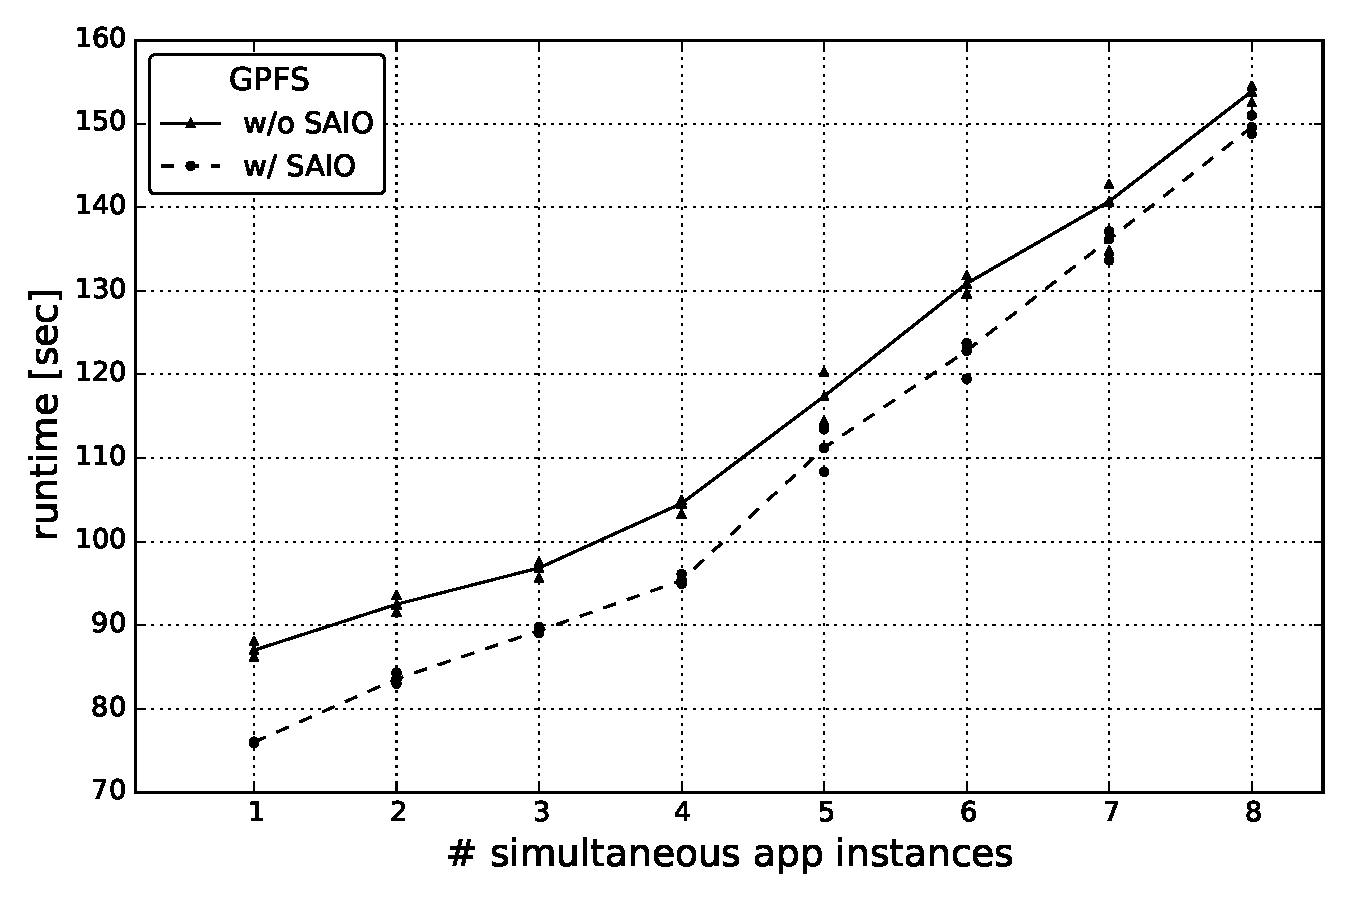
\includegraphics[width=\textwidth]{figures/simult_instance_gpfs_test_cluster}
%    \caption{\textit{}}
%    \label{figure: gpfs_2}
%  \end{subfigure}
%  \begin{subfigure}[b]{0.48\textwidth}
%    \centering
%    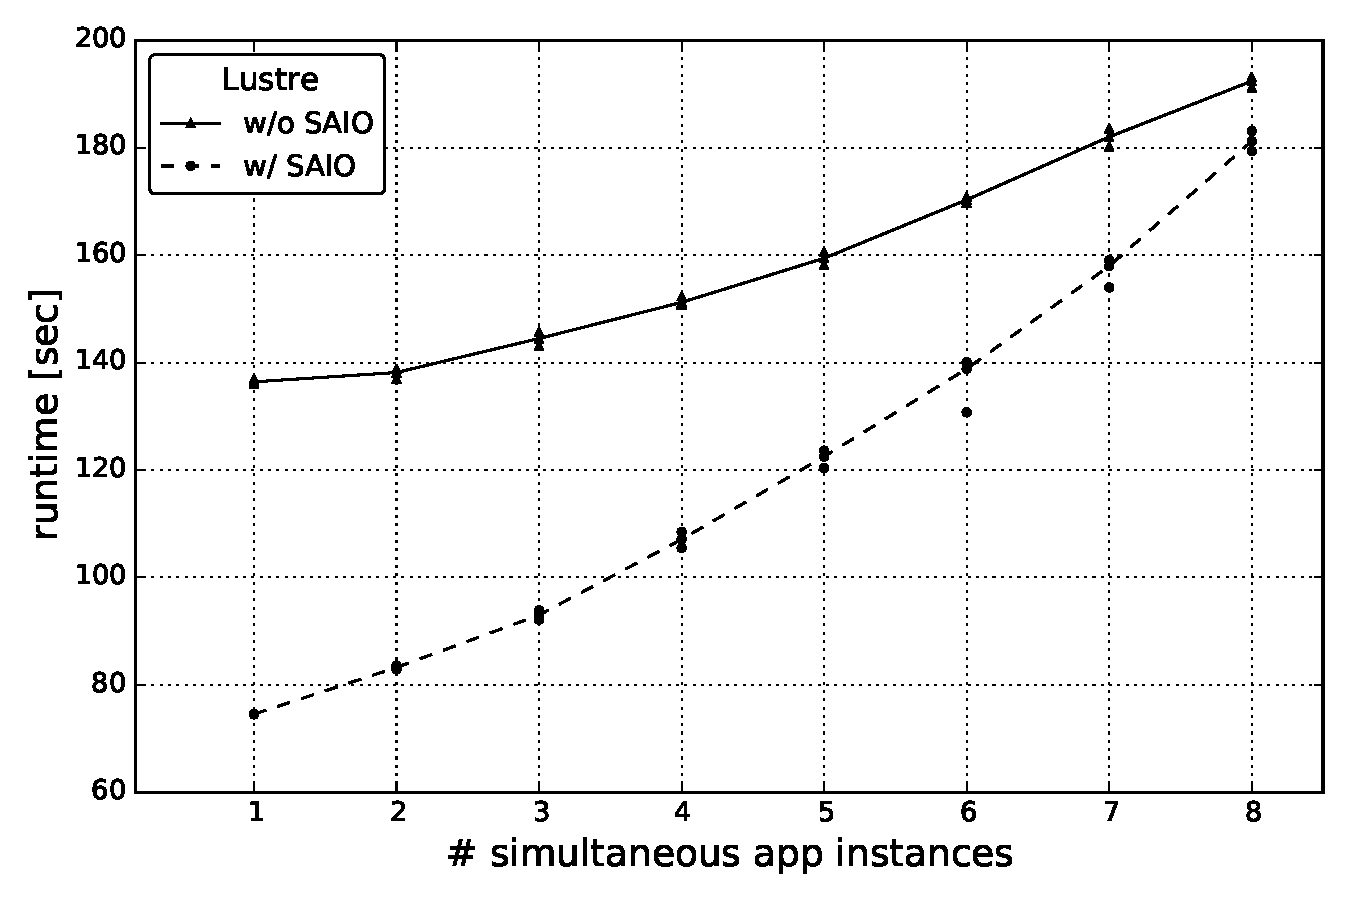
\includegraphics[width=\textwidth]{figures/multiple_simult_procs_Lustre_testcluster}
%    \caption{\textit{}}
%    \label{figure: lustre_2}
%  \end{subfigure}
%  \caption{Running time of the ROOT application for the three file system under study using different of application instances accessing a file of 5 GB (\ref{figure: ext4_2},~\ref{figure: gpfs_2} and~\ref{figure: lustre_2}).}
%  \label{figure: run-time_2}
%\end{figure}
%
%\begin{figure}[!htb]
%  \centering
%  \begin{subfigure}[t]{0.48\textwidth}
%    \centering
%    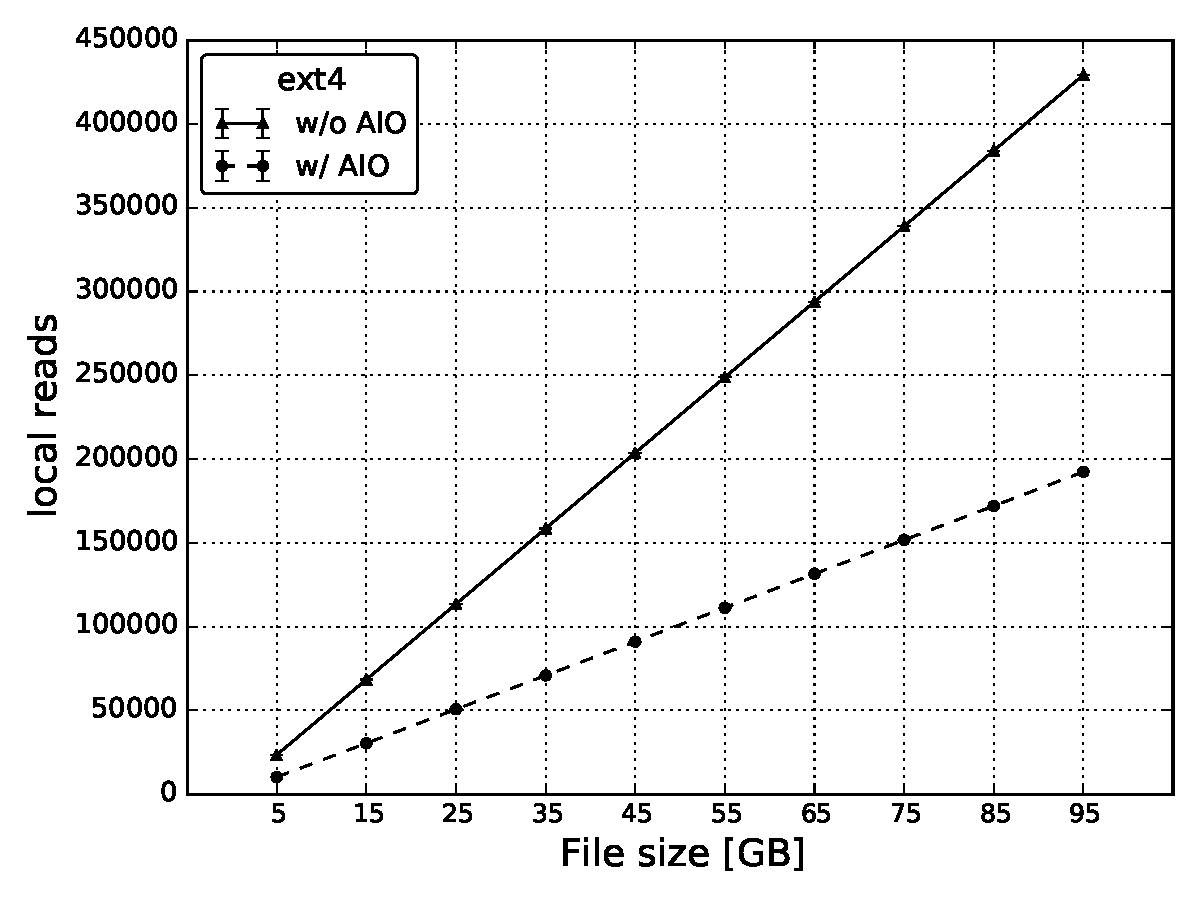
\includegraphics[width=\textwidth]{figures/ext4/reads}
%    \caption{\textit{}}
%    \label{figure: ext4_3}
%  \end{subfigure}
%  \begin{subfigure}[t]{0.48\textwidth}
%    \centering
%    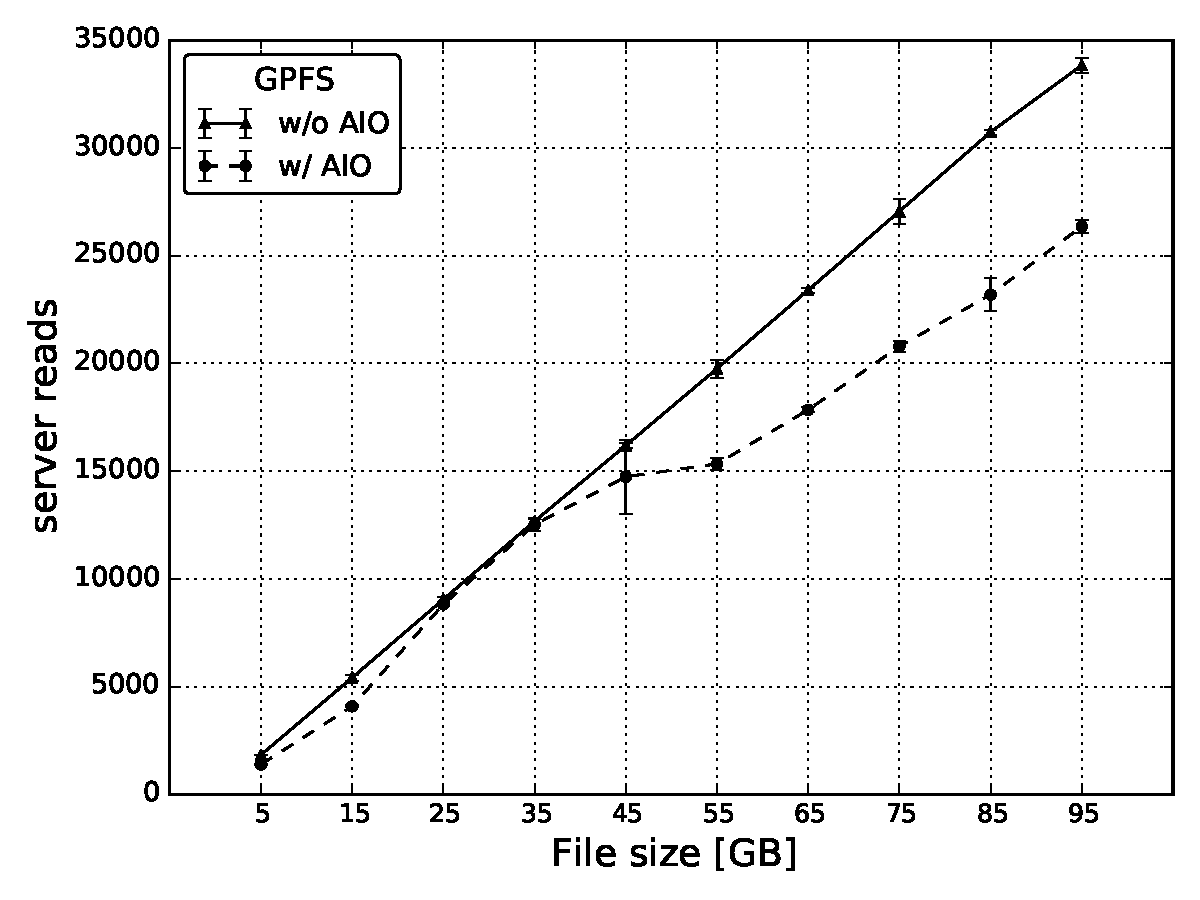
\includegraphics[width=\textwidth]{figures/gpfs/server_reads}
%    \caption{\textit{}}
%    \label{figure: gpfs_3}
%  \end{subfigure}
%  \begin{subfigure}[t]{0.48\textwidth}
%    \centering
%    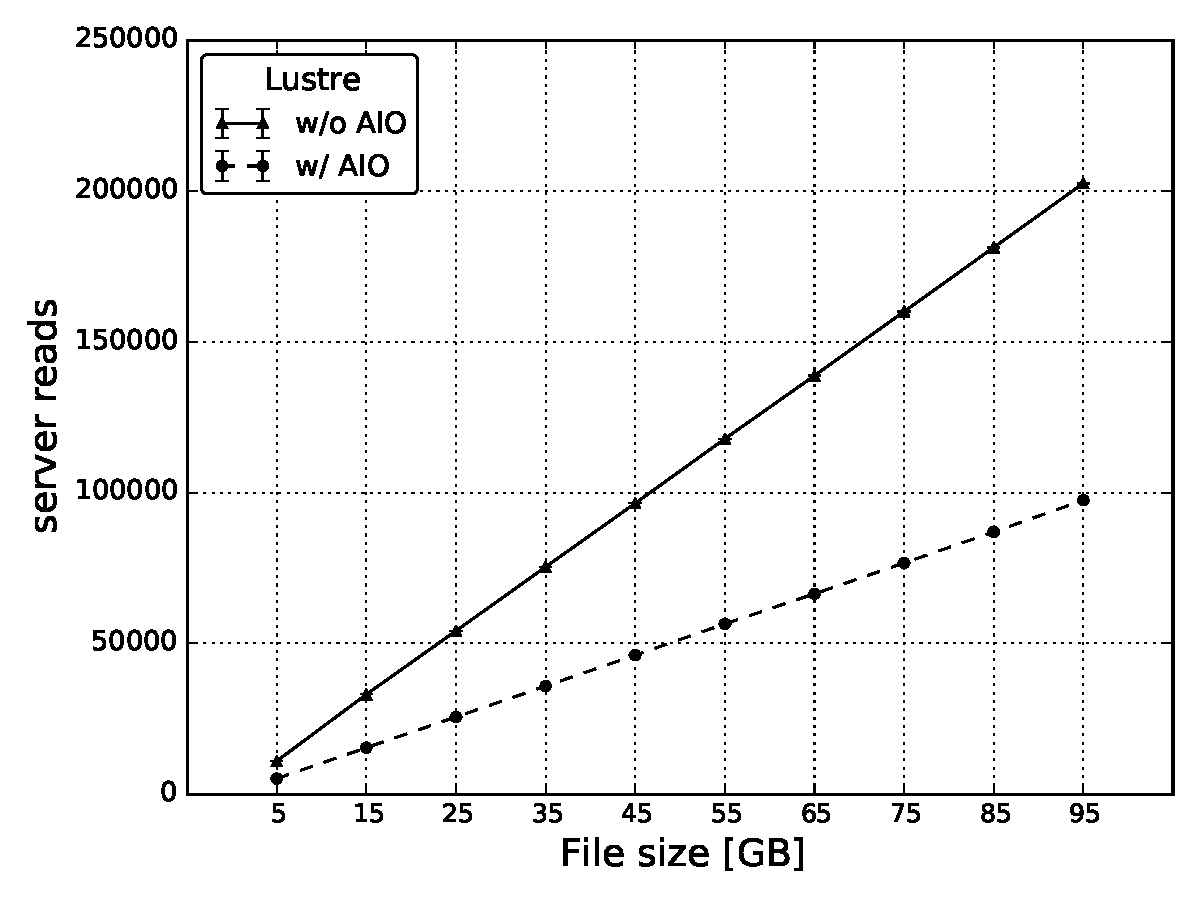
\includegraphics[width=\textwidth]{figures/Lustre/server_reads}
%    \caption{\textit{}}
%    \label{figure: lustre_3}
%  \end{subfigure}
%  \caption{Reads processed by local ext4, GPFS and Lustre I/O servers for various input file sizes (\ref{figure: ext4_3},~\ref{figure: gpfs_3} and~\ref{figure: lustre_3}).}
%  \label{figure: read_1}
%\end{figure}
%
%\begin{figure}[!htb]
%  \centering
%  \begin{subfigure}[b]{0.48\textwidth}
%    \centering
%    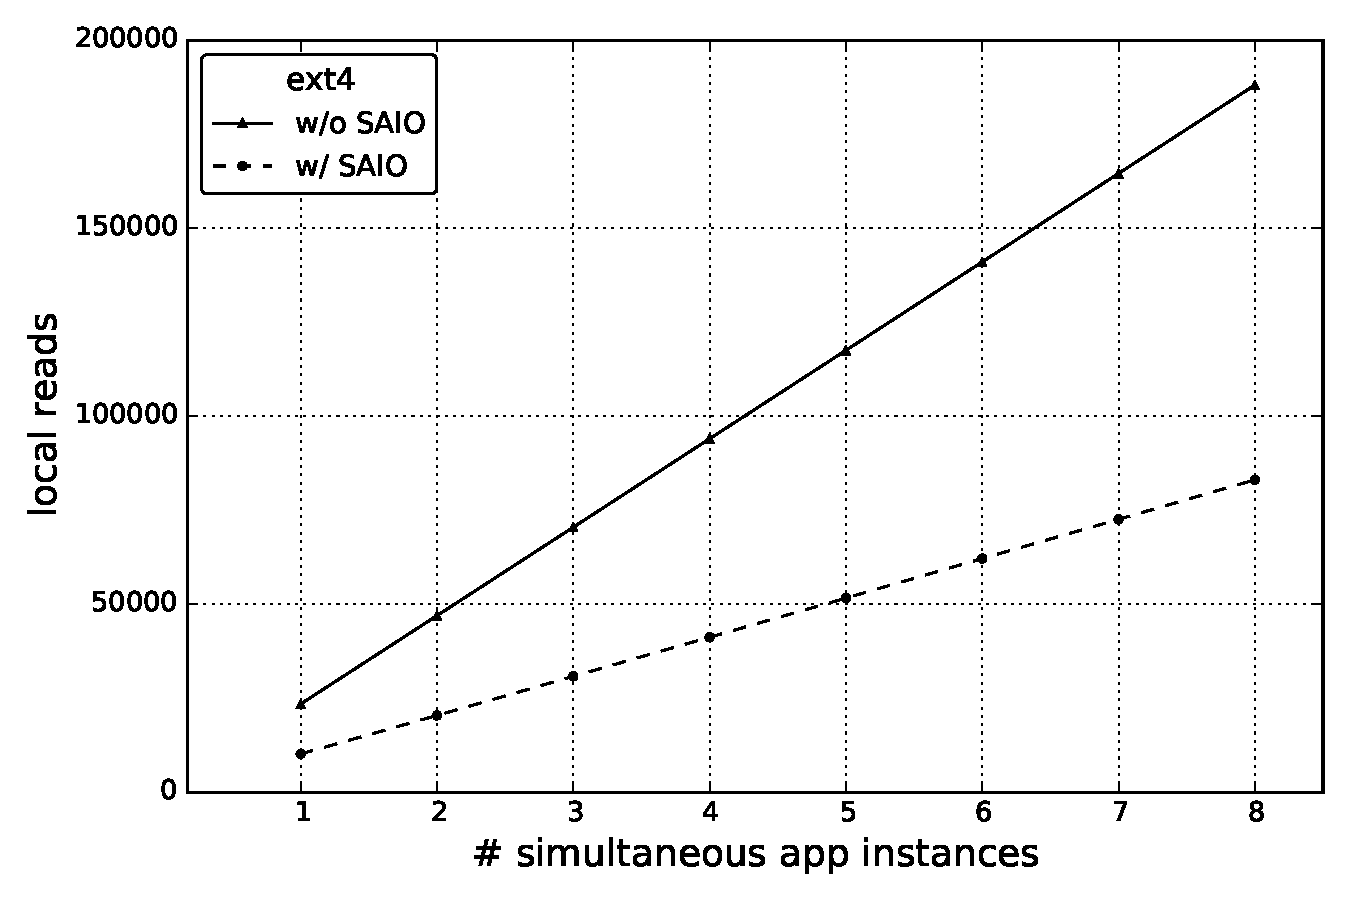
\includegraphics[width=\textwidth]{figures/reads_simult_instance_ext4_test_cluster}
%    \caption{\textit{}}
%    \label{figure: ext4_4}
%  \end{subfigure}
%  \begin{subfigure}[b]{0.48\textwidth}
%    \centering
%    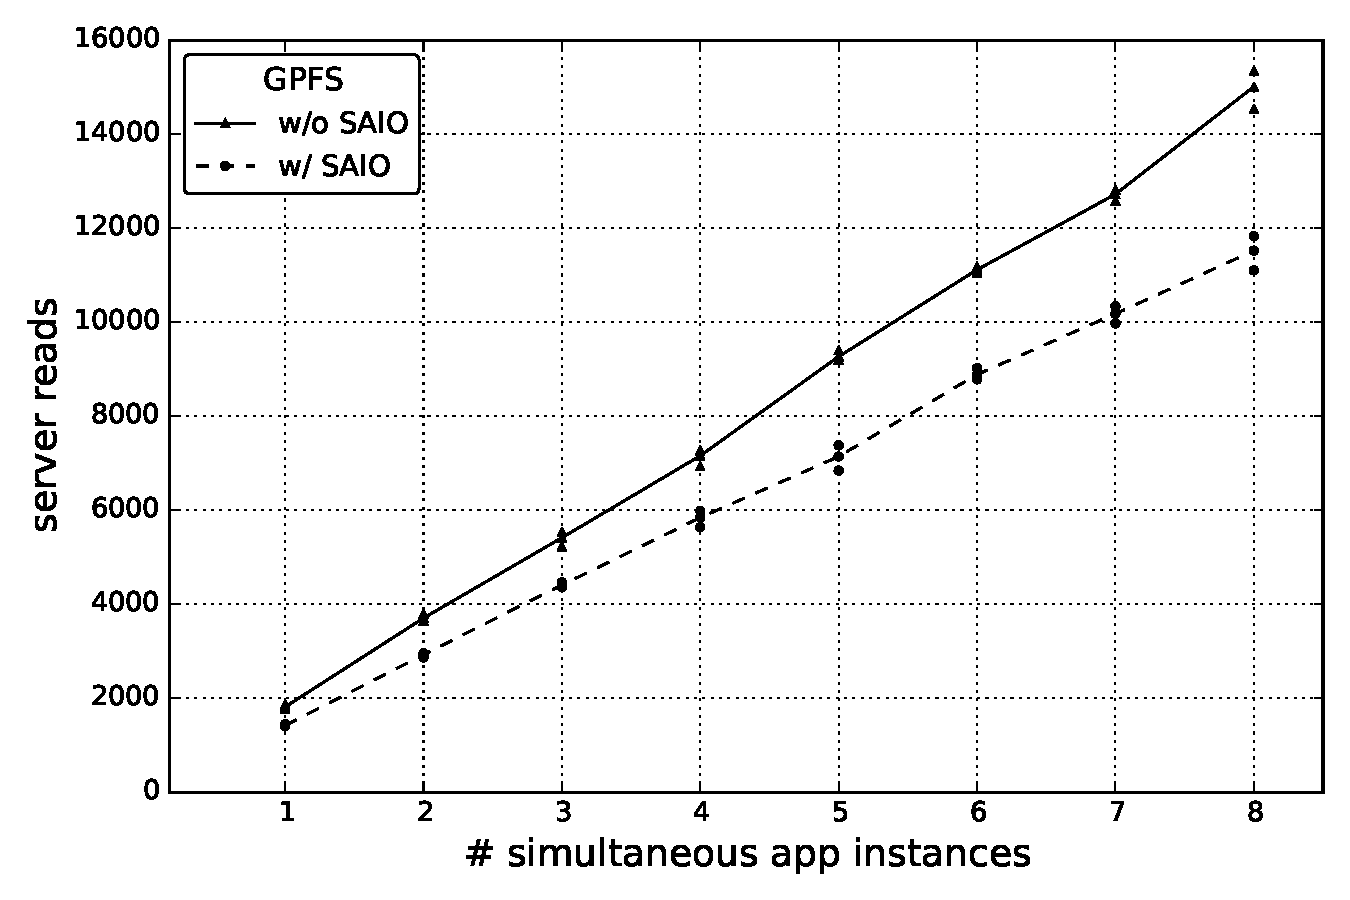
\includegraphics[width=\textwidth]{figures/reads_simult_instance_gpfs_test_cluster}
%    \caption{\textit{}}
%    \label{figure: gpfs_4}
%  \end{subfigure}
%  \begin{subfigure}[b]{0.48\textwidth}
%    \centering
%    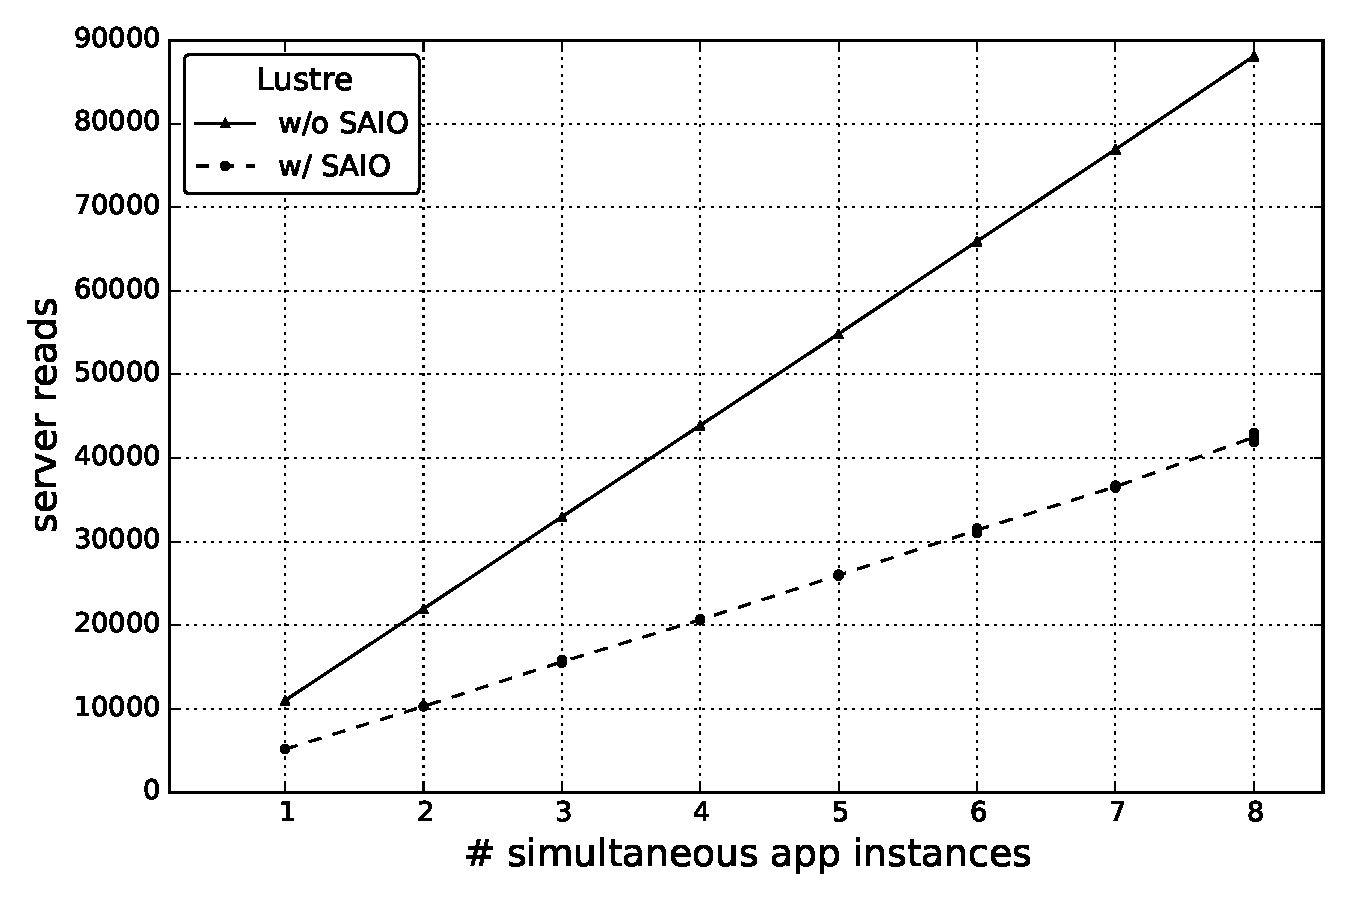
\includegraphics[width=\textwidth]{figures/reads_multiple_simult_procs_Lustre_testcluster}
%    \caption{\textit{}}
%    \label{figure: lustre_4}
%  \end{subfigure}
%  \caption{Reads processed by local ext4, GPFS and Lustre I/O servers for multiple instances of ROOT accessing a file of 5 GB (\ref{figure: ext4_4},~\ref{figure: gpfs_4} and~\ref{figure: lustre_4}).}
%  \label{figure: read_2}
%\end{figure}

\begin{figure*}[]
  \centering
  \begin{subfigure}[]{0.70\textwidth}
    \centering
    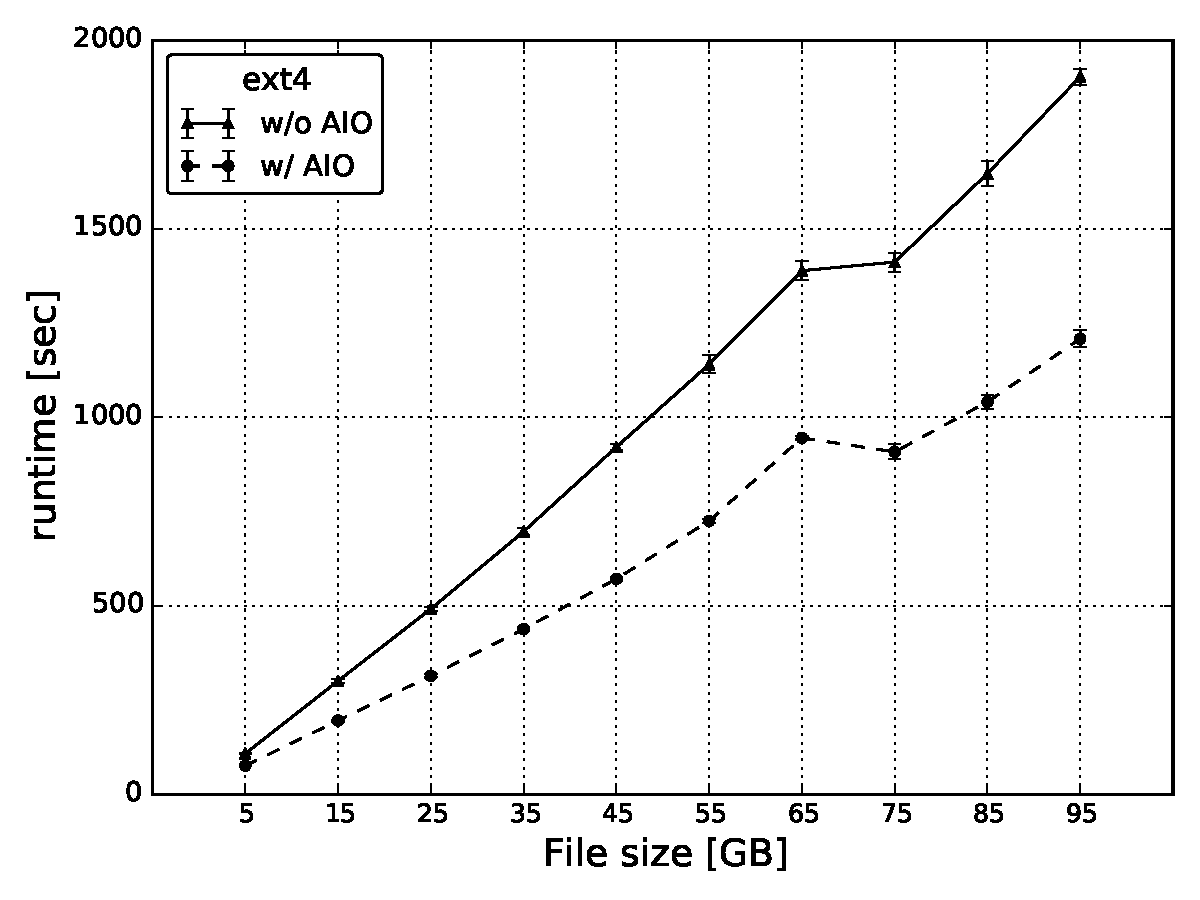
\includegraphics[width=\textwidth]{figures/ext4/runtime}
    \caption{\textit{}}
    \label{figure: ext4_1}
  \end{subfigure}
  \begin{subfigure}[]{0.70\textwidth}
    \centering
    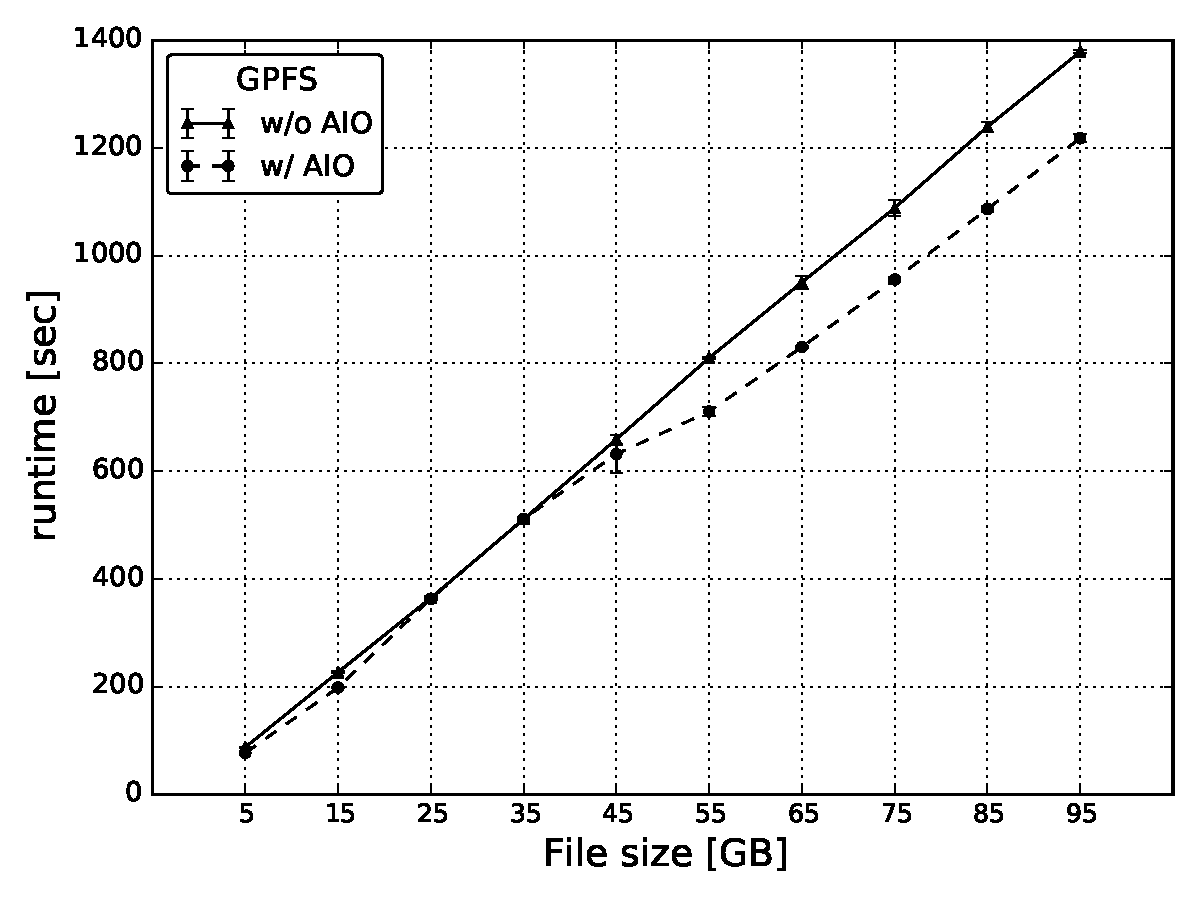
\includegraphics[width=\textwidth]{figures/gpfs/runtime}
    \caption{\textit{}}
    \label{figure: gpfs_1}
  \end{subfigure}
  \begin{subfigure}[]{0.70\textwidth}
    \centering
    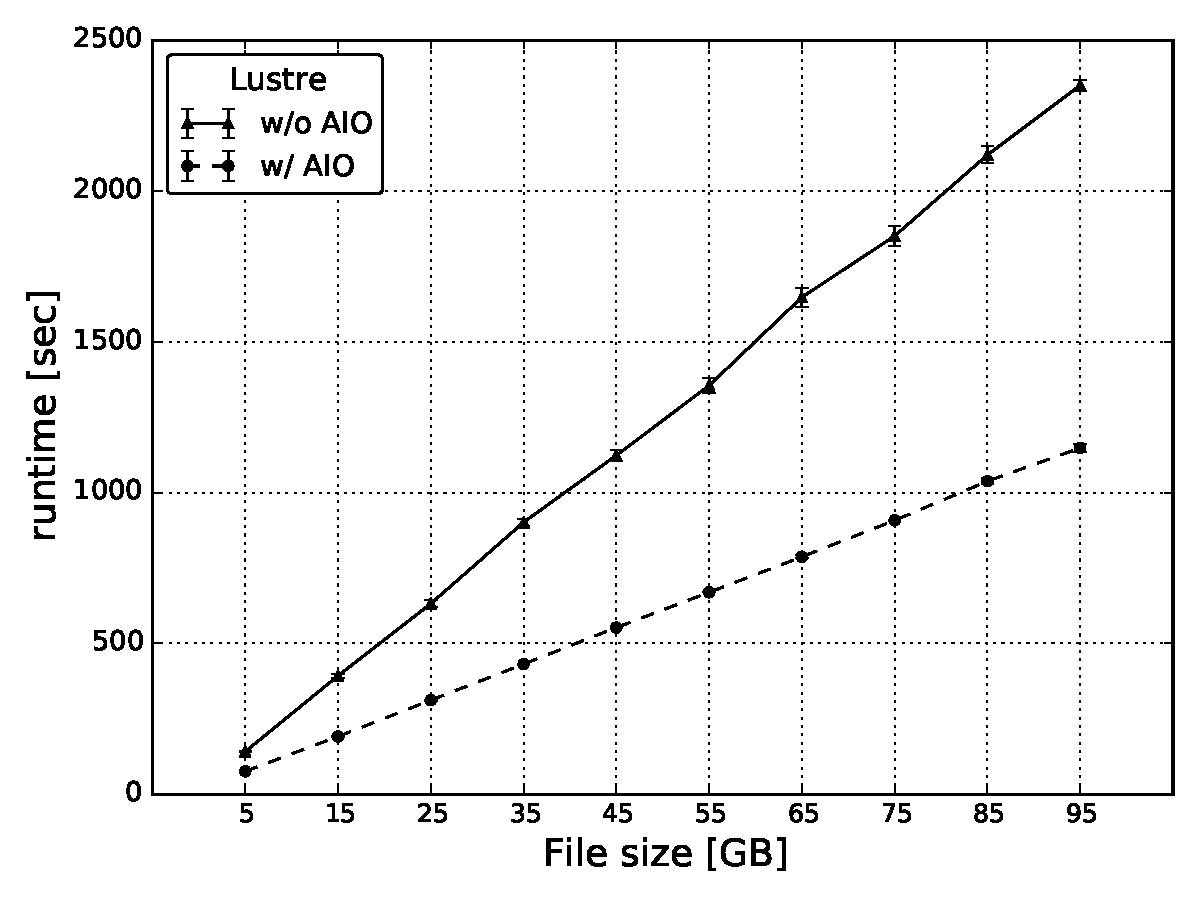
\includegraphics[width=\textwidth]{figures/Lustre/runtime}
    \caption{\textit{}}
    \label{figure: lustre_1}
  \end{subfigure}
  \caption{Running time of the ROOT application for the three file systems under study using different input file sized (\ref{figure: ext4_1},~\ref{figure: gpfs_1} and~\ref{figure: lustre_1}).}
  \label{figure: run-time_1}
\end{figure*}

\begin{figure*}[]
  \centering
  \begin{subfigure}[]{0.70\textwidth}
    \centering
    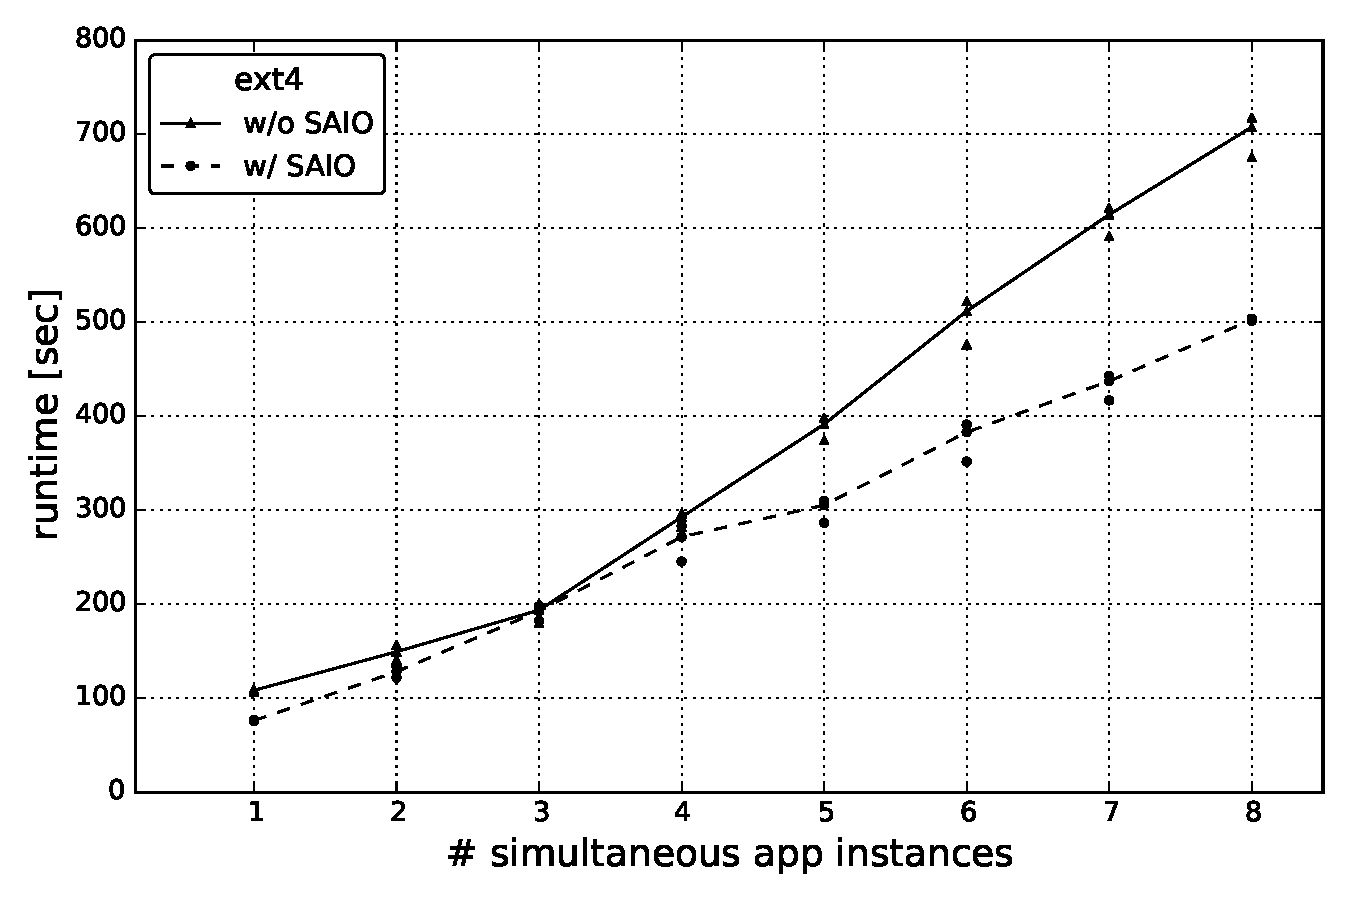
\includegraphics[width=\textwidth]{figures/simult_instance_ext4_test_cluster}
    \caption{\textit{}}
    \label{figure: ext4_2}
  \end{subfigure}
  \begin{subfigure}[]{0.70\textwidth}
    \centering
    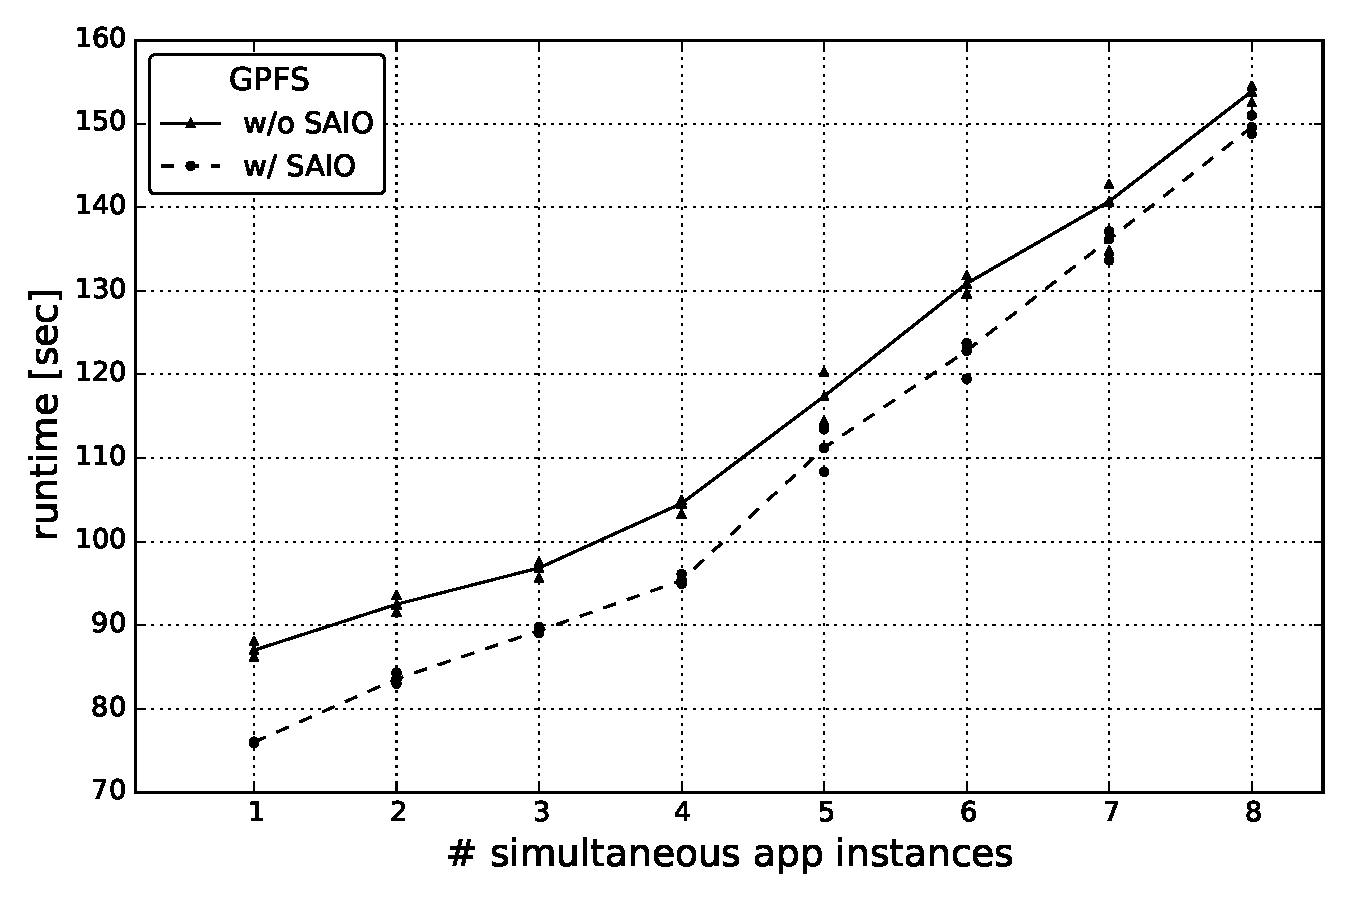
\includegraphics[width=\textwidth]{figures/simult_instance_gpfs_test_cluster}
    \caption{\textit{}}
    \label{figure: gpfs_2}
  \end{subfigure}
  \begin{subfigure}[]{0.70\textwidth}
    \centering
    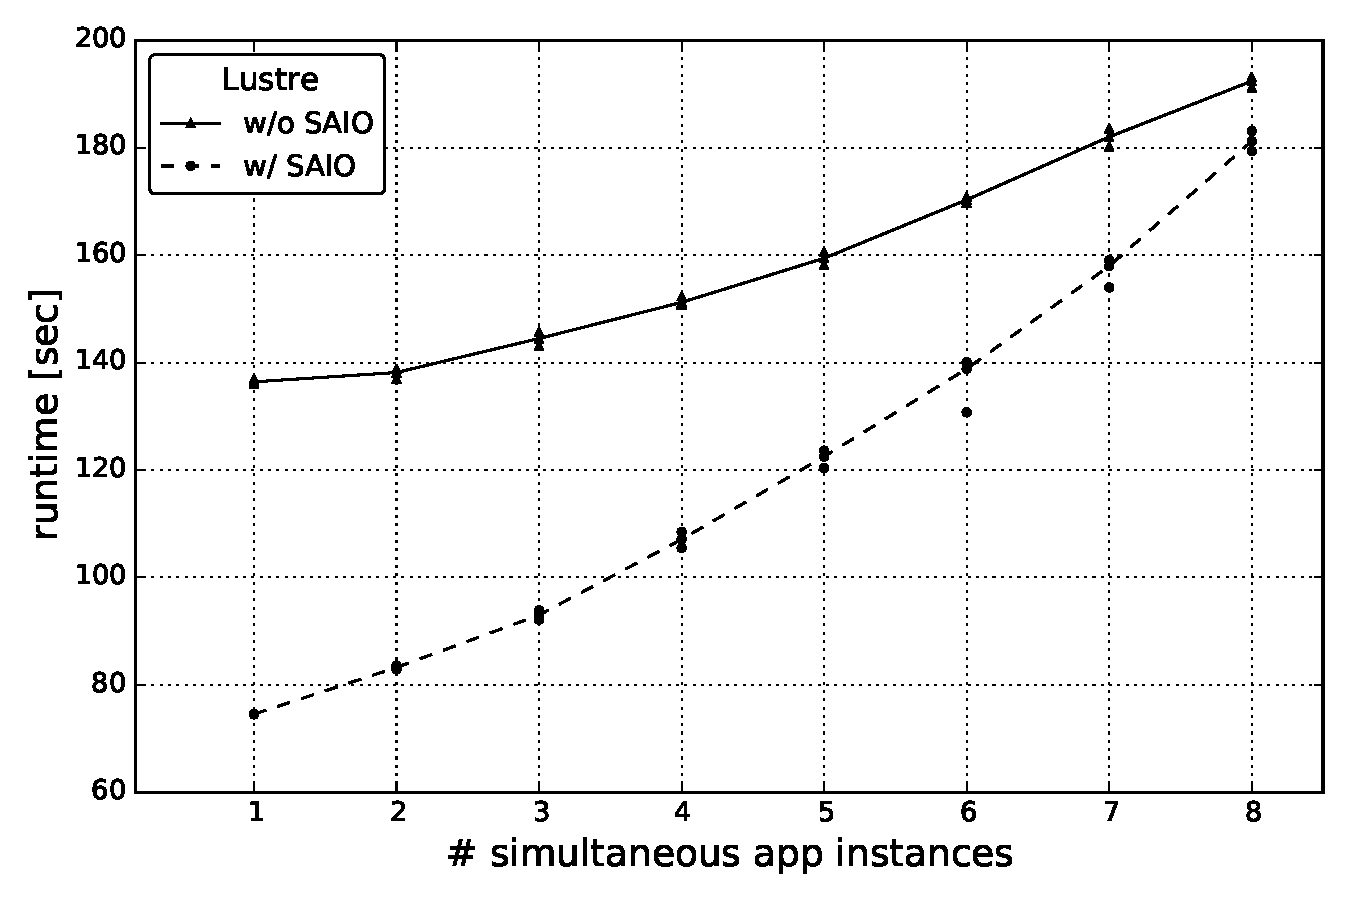
\includegraphics[width=\textwidth]{figures/multiple_simult_procs_Lustre_testcluster}
    \caption{\textit{}}
    \label{figure: lustre_2}
  \end{subfigure}
  \caption{Running time of the ROOT application for the three file system under study using different of application instances accessing a file of 5 GB (\ref{figure: ext4_2},~\ref{figure: gpfs_2} and~\ref{figure: lustre_2}).}
  \label{figure: run-time_2}
\end{figure*}

\begin{figure*}[]
  \centering
  \begin{subfigure}[]{0.70\textwidth}
    \centering
    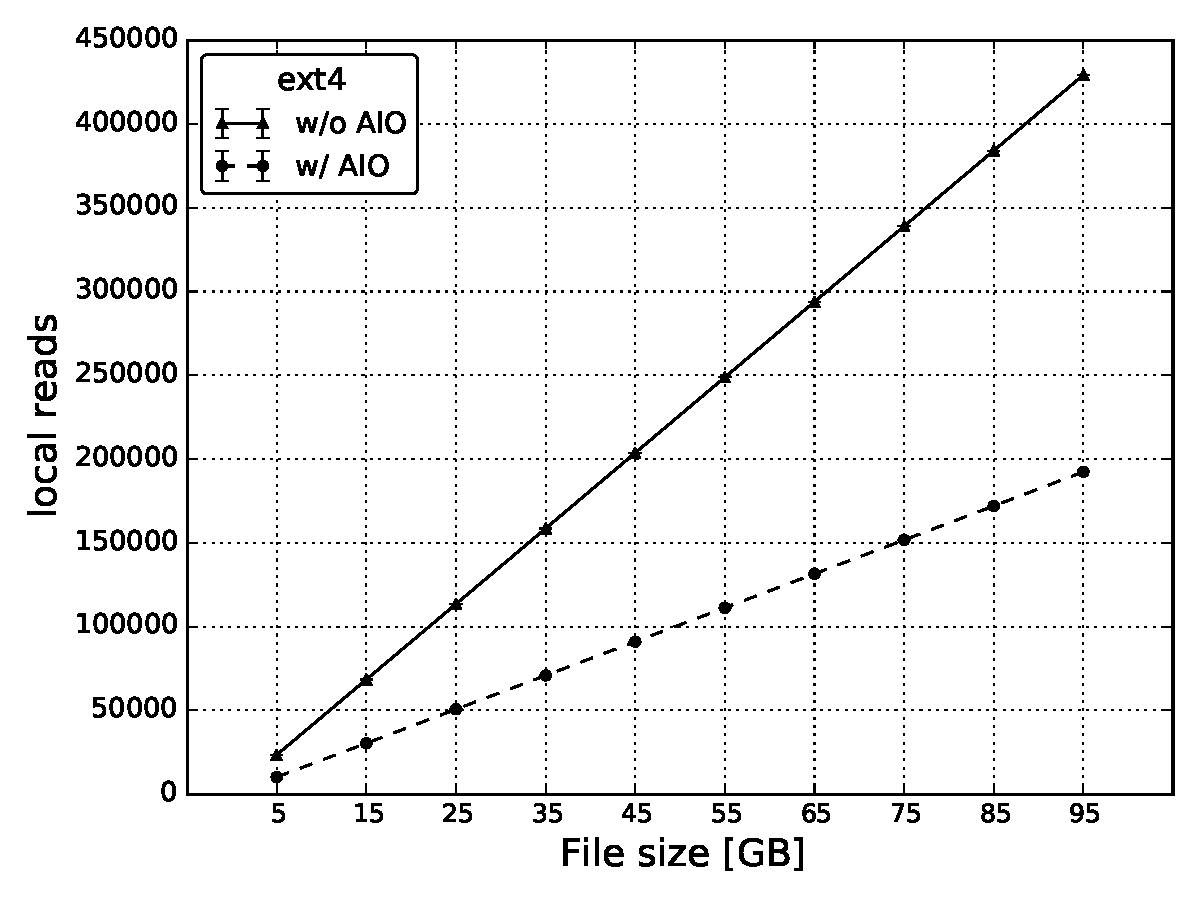
\includegraphics[width=\textwidth]{figures/ext4/reads}
    \caption{\textit{}}
    \label{figure: ext4_3}
  \end{subfigure}
  \begin{subfigure}[]{0.70\textwidth}
    \centering
    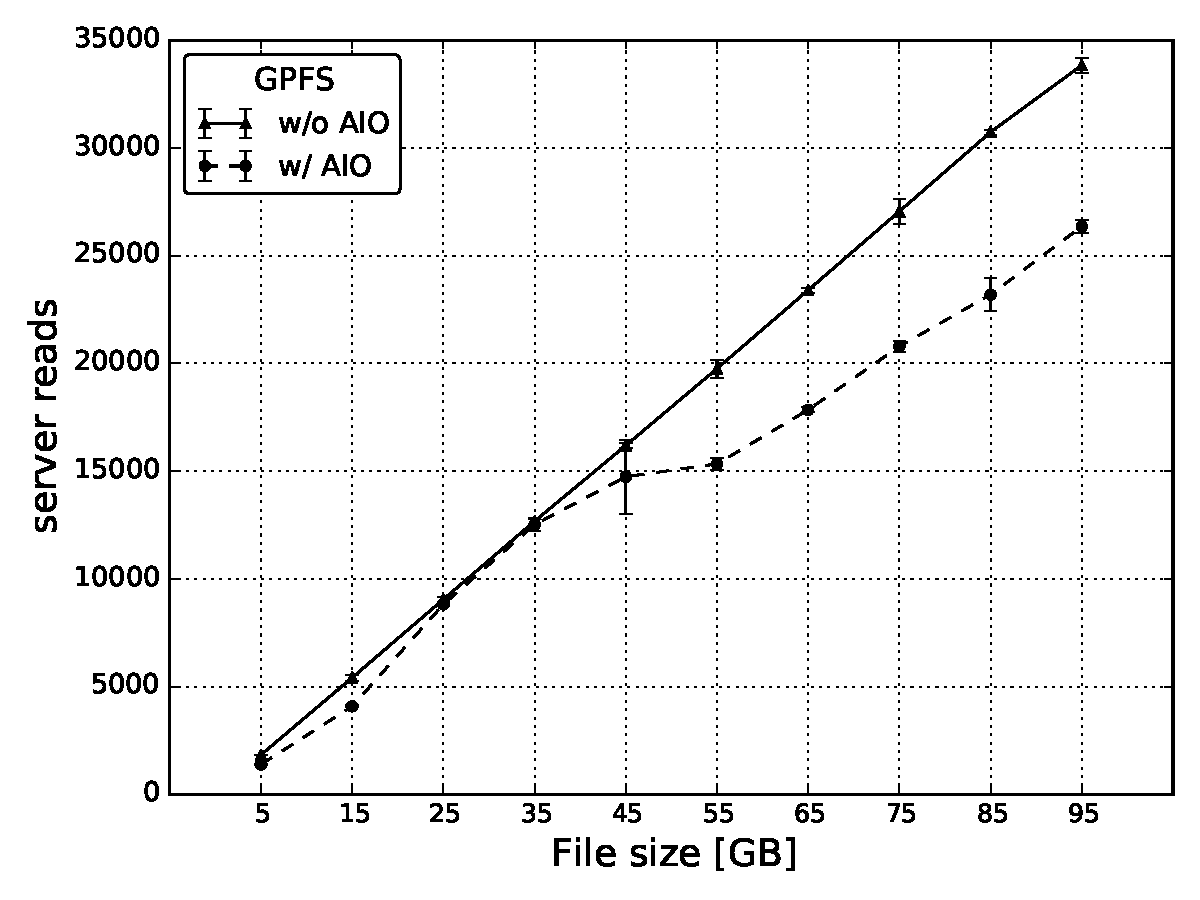
\includegraphics[width=\textwidth]{figures/gpfs/server_reads}
    \caption{\textit{}}
    \label{figure: gpfs_3}
  \end{subfigure}
  \begin{subfigure}[]{0.70\textwidth}
    \centering
    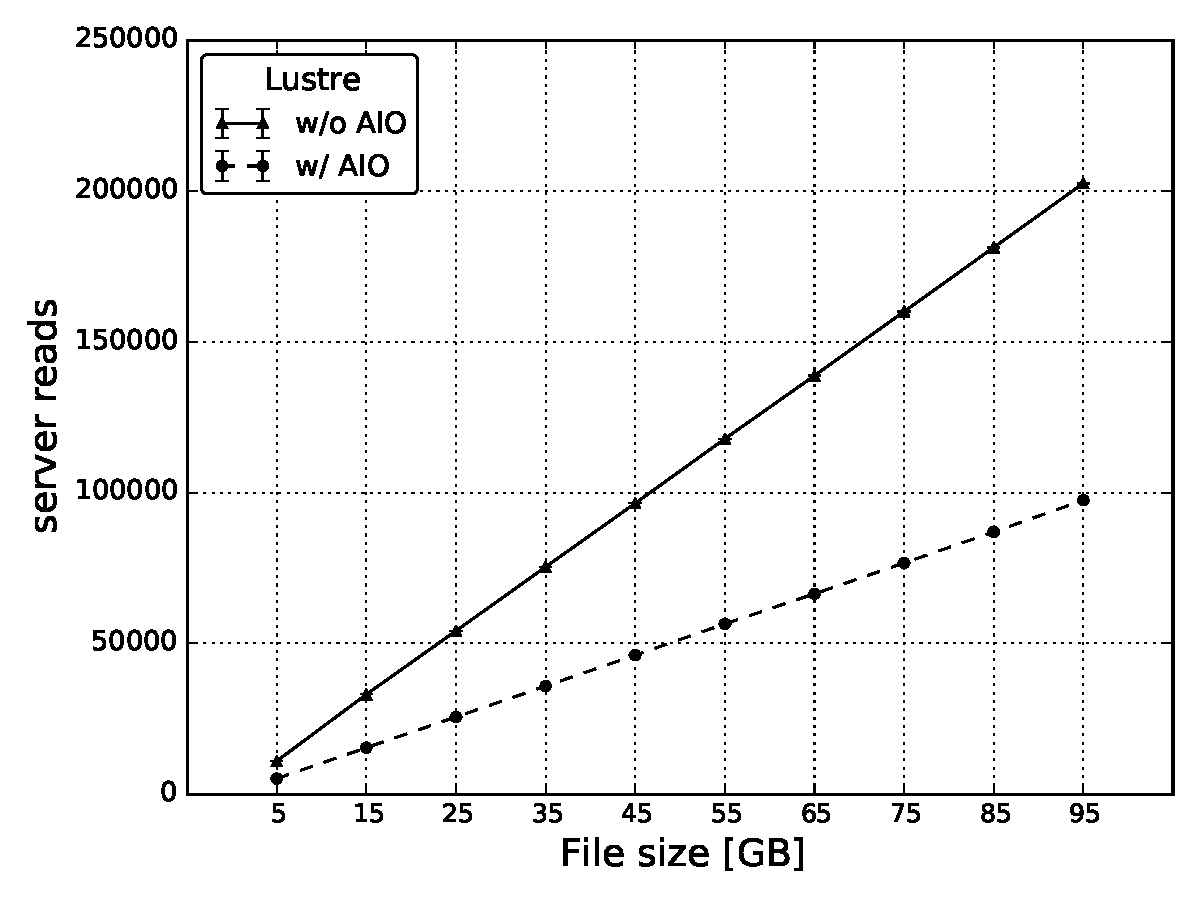
\includegraphics[width=\textwidth]{figures/Lustre/server_reads}
    \caption{\textit{}}
    \label{figure: lustre_3}
  \end{subfigure}
  \caption{Reads processed by local ext4, GPFS and Lustre I/O servers for various input file sizes (\ref{figure: ext4_3},~\ref{figure: gpfs_3} and~\ref{figure: lustre_3}).}
  \label{figure: read_1}
\end{figure*}

\begin{figure*}[]
  \centering
  \begin{subfigure}[]{0.70\textwidth}
    \centering
    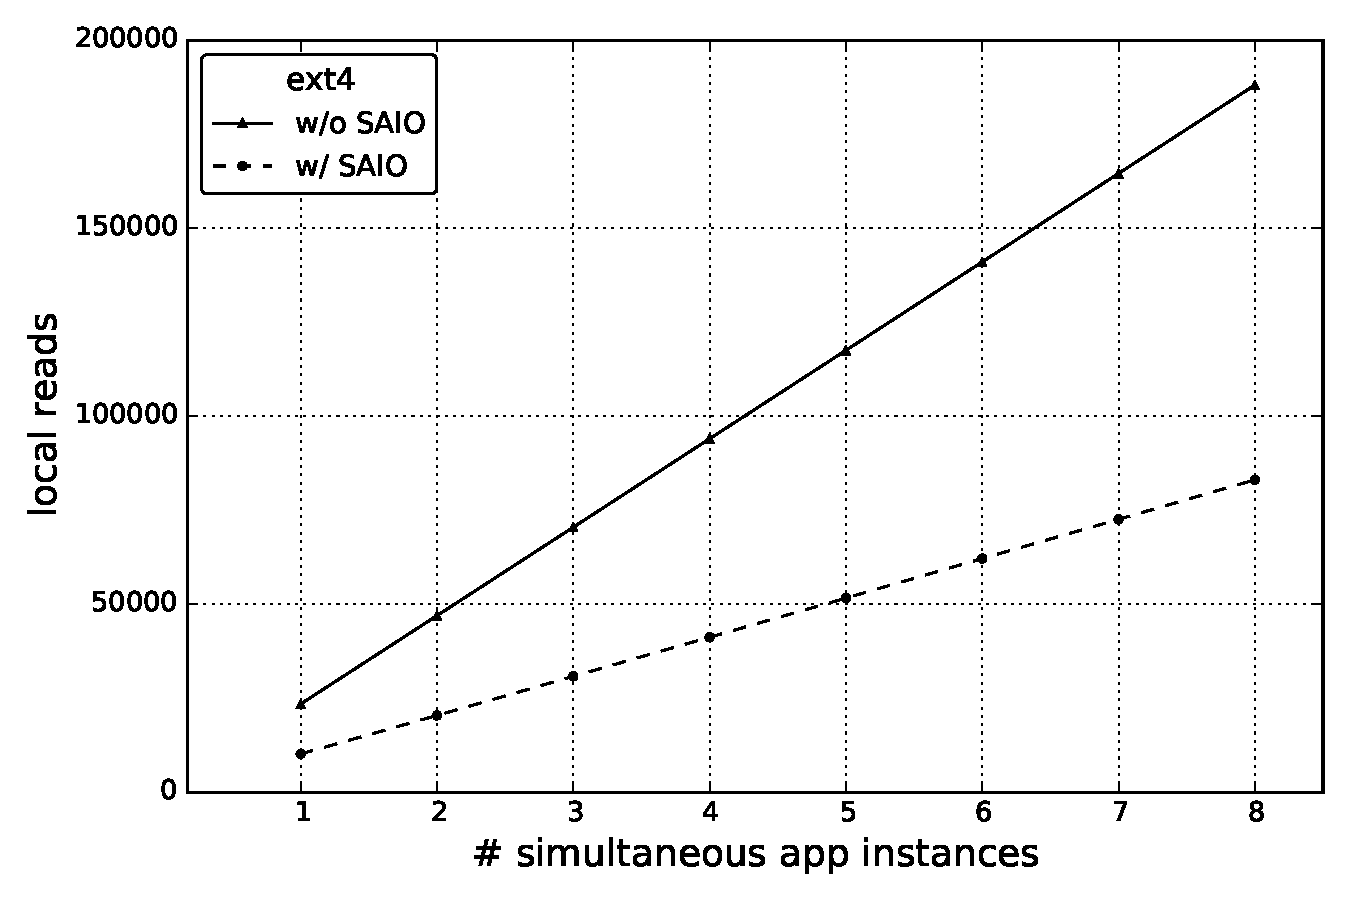
\includegraphics[width=\textwidth]{figures/reads_simult_instance_ext4_test_cluster}
    \caption{\textit{}}
    \label{figure: ext4_4}
  \end{subfigure}
  \begin{subfigure}[]{0.70\textwidth}
    \centering
    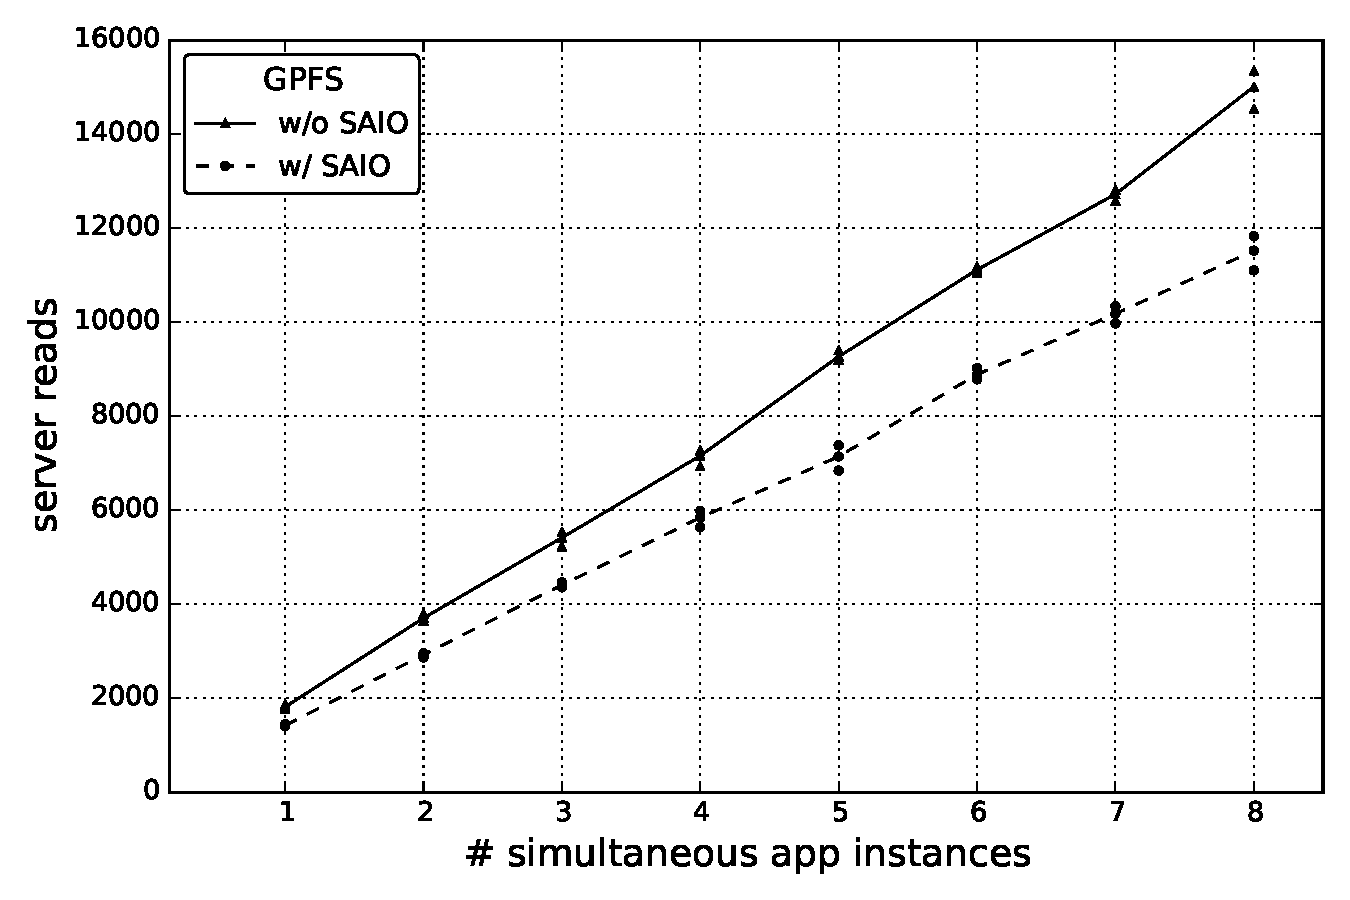
\includegraphics[width=\textwidth]{figures/reads_simult_instance_gpfs_test_cluster}
    \caption{\textit{}}
    \label{figure: gpfs_4}
  \end{subfigure}
  \begin{subfigure}[]{0.70\textwidth}
    \centering
    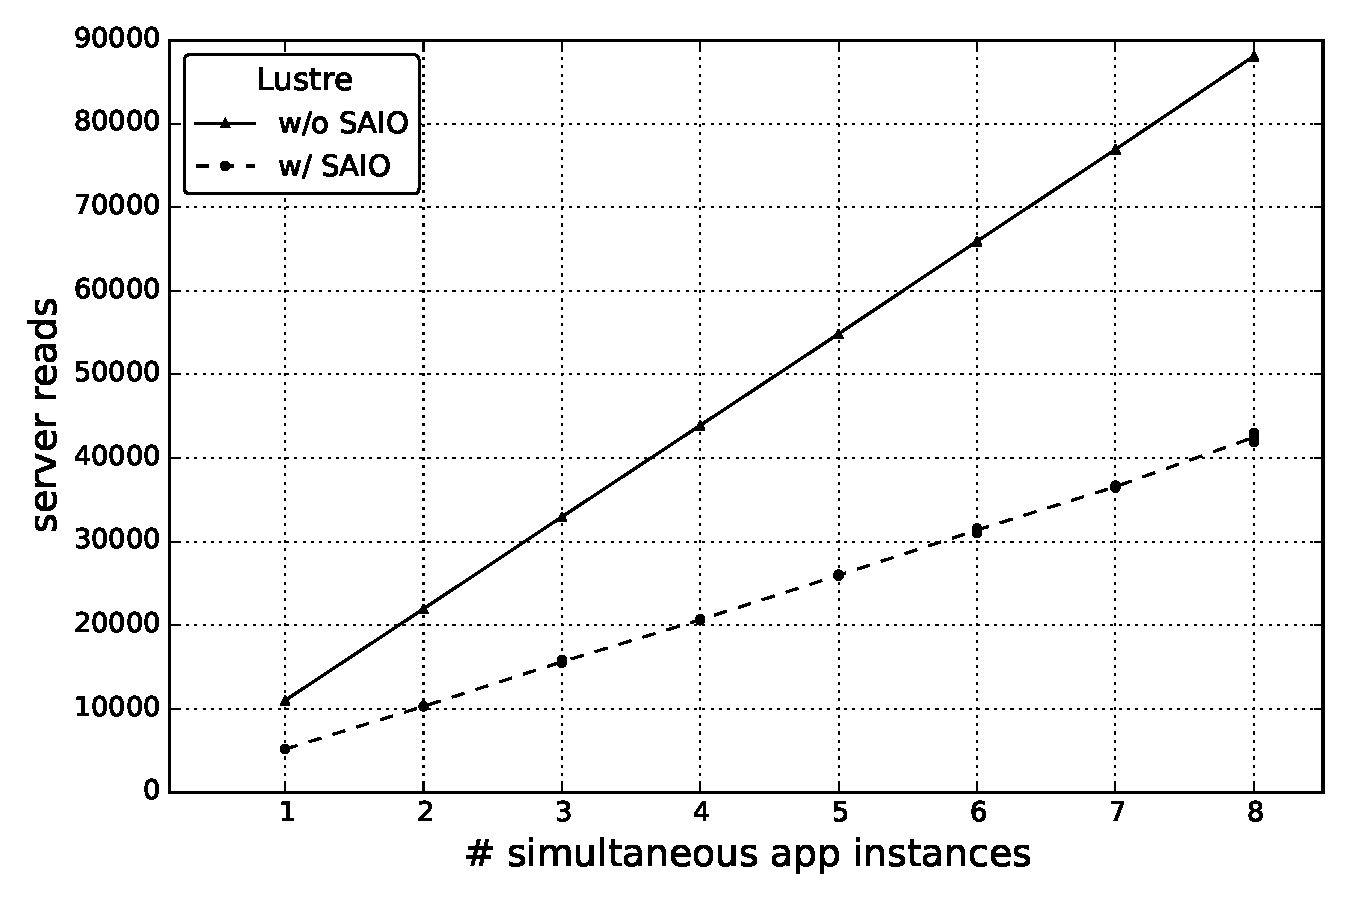
\includegraphics[width=\textwidth]{figures/reads_multiple_simult_procs_Lustre_testcluster}
    \caption{\textit{}}
    \label{figure: lustre_4}
  \end{subfigure}
  \caption{Reads processed by local ext4, GPFS and Lustre I/O servers for multiple instances of ROOT accessing a file of 5 GB (\ref{figure: ext4_4},~\ref{figure: gpfs_4} and~\ref{figure: lustre_4}).}
  \label{figure: read_2}
\end{figure*}

As far as Figures~\ref{figure: ext4_2},~\ref{figure: gpfs_2} and~\ref{figure: lustre_2} are concerned, these account for the effect of processes' concurrency on the file system. 
Before continuing with the discussion we have to make a note here. In our architecture, only one process per file system's client issues (through multiple \textit{Advisor Thread}s) 
hints on behalf of running applications. This introduces some overhead, since we have to pass the access information from the \textit{Assisted I/O library} to the \textit{Advice Manager}, 
but has the advantage of better coordinating accesses to the same file from multiple processes. Nevertheless, we found that in the case of GPFS, despite the fact of having multiple 
\textit{Advisor Thread}s, only one process among the many was receiving a benefit from the prefetching hints; the reason is that GPFS seems to have the restriction of hinting only one 
file per process. For this reason, we developed another variant of Mercury in which the AIO library, now renamed \textit{Self Assisted I/O library} (SAIO), internally provides the 
creation and the handling of multiple \textit{Advisor Thread}s. 

Looking at the figures generated with the new SAIO library we can assess the effectiveness of the prefetching hints for 
the three file systems considered. In particular, Lustre provides the best run-time improvements compared to the case in which no hints were used. GPFS shows a more contained improvement 
since the I/O time is already small compared to Lustre and ext4. Finally, ext4 can really benefit from prefetching hints especially for high process counts. Overall, excluding ext4, when 
we increase the number of processes the run-time improvements shrink. Because ext4 transfers data directly from the local SATA HDD, in which I/O time is dominated by disk latency, we can 
still improve performance as the number of application instances increases by making efficient use of the cache to hide such latency. GPFS and Lustre servers, on the other hand, have much 
higher transfer performance compared to single disk ext4 and both use a network link to move data across the network; GPFS uses the NSD protocol while Lustre uses the LNET protocol. For GPFS
and Lustre network bandwidth becomes critical and, in fact, as the number of instances increases the run-time decreases because of the saturation of the network link in the node.

Figure~\ref{figure: ext4_3},~\ref{figure: gpfs_3} and~\ref{figure: lustre_3} report the number of read requests accounted for by the different file systems under study. More specifically, 
the figures show how the number of reads at the I/O server side for both GPFS and Lustre can be substantially reduced with our approach. This has a significant impact in HPC cluster in 
which the file system may be accessed by many thousand of processes at the same time. Reducing the number of requests for an application can increase the number of IOPS available for others. 
This result is also confirmed for multiple instances of the `ROOT' application running concurrently (Figure~\ref{figure: ext4_4},~\ref{figure: gpfs_4} and~\ref{figure: lustre_4}).

\subsection{Conclusions}
Our experiments have focused on prefetching performance in a real scenario setup. In particular we have considered the cache utilization by a single application's instance as well as the
combined cache utilization by multiple application's instances. We have shown how in both cases we can reduce the application runtime by aggressively prefetching data into main memory using
our transparent approach. However, since our strategy is bandwidth bound we have seen that in the case of multiple application's instances such approach leads to the saturation of the
network link in the case of networked file systems and ultimately to the shrinking of the performance gain.

%One important aspect to consider in HPC is that although nodes typically run only a single application at a time, there might
%be still multiple instances of it operating on different parts of the input dataset (SPMD model). As we have mentioned in Chapter~\ref{chapt: introduction} the number of cores in HPC nodes
%is increasing faster than the amount of available memory per core. This, combined with the fact that prefetching performance are limited by the saturation of the network link in the case of
%intense I/O activity, poses a further criticality on optimal cache management policies. In this sense, our solution provides effective control over the cache utilization to the user, that can
%thus make sure that unneeded pages are explicitly evicted from the cache using hints, saving up space for more valuable pages and reducing the network traffic from the network file system.

\section{Write Behind in Collective I/O}
To evaluate the proposed MPI-IO hints we use three popular I/O benchmarks frequently adopted to profile collective I/O performance in other research works: 
coll\_perf\footnote{Collective I/O benchmark distributed with the MPICH package.}, Flash-IO and IOR. The main difference between these three benchmarks is 
the amount of data written per I/O and access pattern. In fact, coll\_perf writes all the strided data (32~GB) in a single collective I/O operation using 
\texttt{MPI\_File\_write\_all()}, Flash-IO writes small amounts of strided data (in the order of few MB) over multiple collective I/O operations using 
\texttt{MPI\_File\_write\_at\_all()}, and finally IOR writes larger amounts of contiguous data than Flash-IO (4~GB) over multiple collective I/O operations.

Minor changes to the source code of the three benchmarks have been made to adapt them to our needs. For example, coll\_perf and Flash-IO did not support writing 
to multiple files or the emulation of computing time between writes. Thus, we modified them to reproduce a workflow similar to the one shown in Figure~\ref{figure: workflow}. 
The number of written files and a compute time are now parameters that can be passed from the command line. In all our tests we used 512 MPI processes distributed over 
64 nodes (8 procs/node), fixed the file stripe size to 4~MB and the stripe count to 4. Moreover, for simplicity, we also fixed the size of the cache synchronisation 
buffer (i.e. \codeword{ind\_wr\_buffer\_size}) to 512~KB, which corresponds to the standard independent I/O buffer size. On the other hand, we varied the collective 
I/O parameters, i.e., the number of aggregators (from 8 to 64) and the collective buffer size (from 4~MB to 64~MB). 
For every combination of the described parameters (<aggregators>\_<coll\_bufsize>) each benchmark writes four files of the same size (32~GB) with a compute delay of 30 seconds, 
which is in most cases enough to hide the synchronisation time. We compute the bandwidth as the average bandwidth over the four collective write operations (Equation~\ref{formula: abw}). 

The different contributions within the collective I/O write path shown in Figure~\ref{figure: coll_io_impl} are extracted from the ROMIO layer using MPE profiling
~\cite{Gropp2014}. Whenever the compute delay is not enough to hide synchronisation cost (e.g. when a small number of aggregators is used), the remaining synchronisation 
time is added to the total write time, thus reducing the bandwidth.

\subsection{Testbed}
Our testbed is a research cluster designed and developed in the context of the DEEP/-ER~\cite{Eicker2013} projects (Dynamic Exascale Entry Platform/-Extended Reach). The 
DEEP/-ER cluster has 2048 cores distributed over 128 computing nodes (dual socket Sandy Bridge architecture). The storage system is composed of 6 Dell PowerEdge 
R520 servers equipped with 2 Intel Xeon Quad-core CPUs and 32~GB of memory and run the BeeGFS file system from Fraunhofer ITWM~\cite{Mcpeek2002}
(formerly known as FhGFS). The servers are connected to a SGI JBOD with 45 2TB SAS drives through a SAS switch using two 4x ports at 6~GB/s, for a total of four 
8+2 RAID6 storage targets and 2 RAID1 targets for metadata and management data (1 drive is left as spare). One of the six I/O servers is dedicated as metadata 
server, one as management server and the remaining four as data I/O servers.
Additionally, every compute node is equipped with 32~GB of RAM memory and a 80~GB SATA SSD containing the operating system plus an additional 30~GB ext4 partition 
(mounted under `/scratch') for general purpose storage. This partition, in our case, is used to locally cache collective writes. Finally, all the computing nodes 
are connected through an Infiniband QDR network and use ParaStation MPI\footnote{\url{http://www.par-tec.com/products/parastation-mpi.html}.} (PSMPI) version 5.1.0-1 
as message passing library.

\subsection{Performance Results}
We measured collective I/O performance using Formula~\ref{formula: bw} and~\ref{formula: abw} for the application perceived bandwidth. Additionally, we also measured
the effect of the single ext2ph contributions to collective I/O, as reported in Figure~\ref{figure: coll_io_impl}. In the rest of this section we present our findings
for the three target benchmarks.

\subsubsection{Coll\_perf}
Coll\_perf is a synthetic benchmark that performs collective I/O to a shared file using a single collective write operation. The application uses a three-dimensional
dataset partitioned and assigned to available processes using a block-block strategy~\cite{Bordawekar1993}, that is, the original input domain is divided into a number of blocks equal to the 
number of processes, and each is assigned to a process. Each block is afterwards written to the file using a row-major order. In our configuration we use 512 processes 
distributed over 64 nodes of the 128 available in the DEEP cluster. Every process handles a block with $256 \times 256 \times 256$ integer elements, for a total 64~MB of data
per process and 32~GB for the whole file.

In our experiments we measured three values of write bandwidth: 

\begin{itemize}
\item the bandwidth when the cache is disabled (this is the default case) and collective I/O writes data to the global file system directly (\textit{BW Cache Disable}); 
\item the bandwidth when the cache is enabled and data is flushed immediately to the global file system (\textit{BW Cache Enable}); and 
\item the bandwidth when the cache is enabled but data is not flushed to the global file system (\textit{TBW Cache Enable}). 
\end{itemize}

The latter gives us a theoretical bandwidth figure (TBW) that we can use to estimate how well the cached collective I/O implementation is doing. In order to measure the potential 
benefits of our cached approach we modify the workflow in Figure~\ref{figure: workflow} moving the write phase before the compute phase. In this way we can always overlap cache 
synchronization with compute.

\begin{figure*}[]
  \centering
  \begin{subfigure}[]{0.7\textwidth}
  \centering
  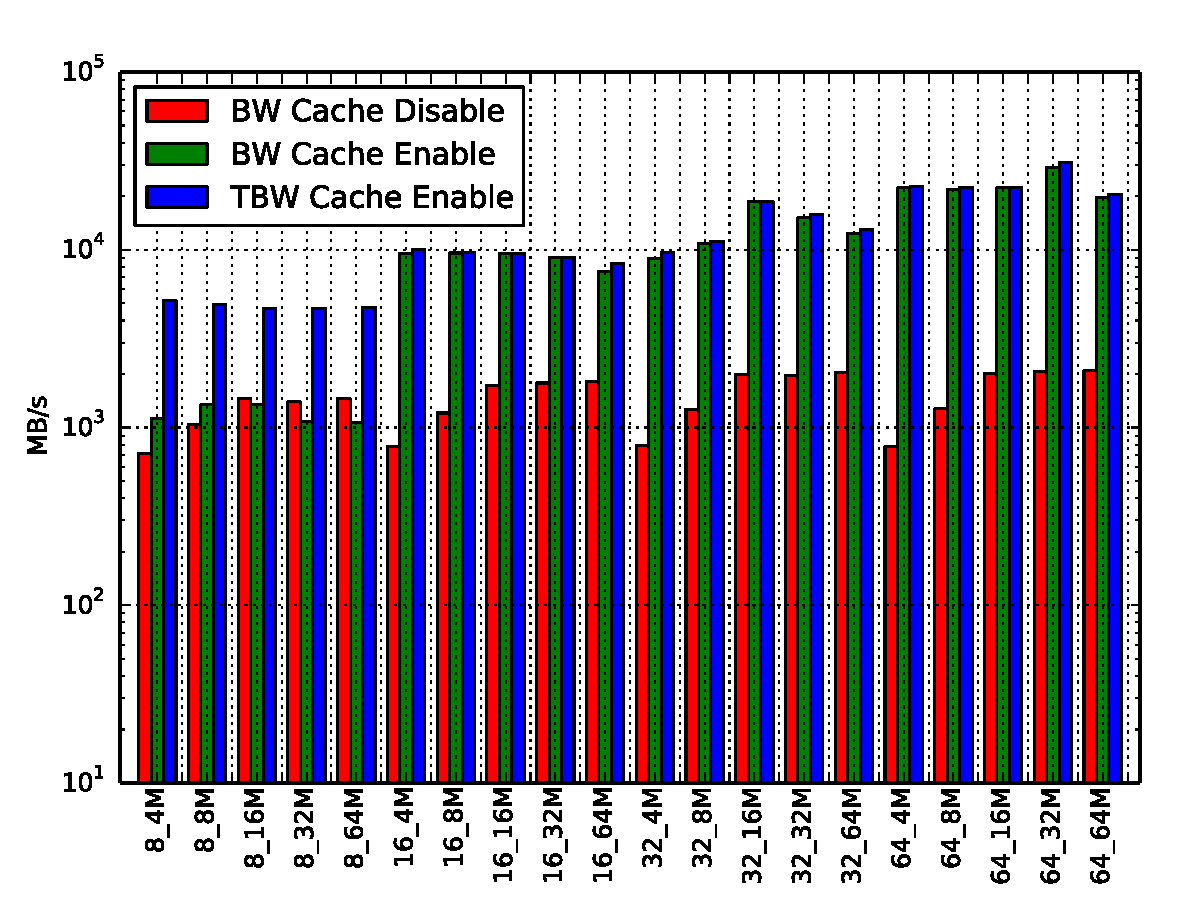
\includegraphics[width=\textwidth]{figures/coll_perf_32GB_30sec_bw}
  \caption{}
  \label{figure: collperf-bw}
  \end{subfigure}
  \begin{subfigure}[]{0.7\textwidth}
  \centering
  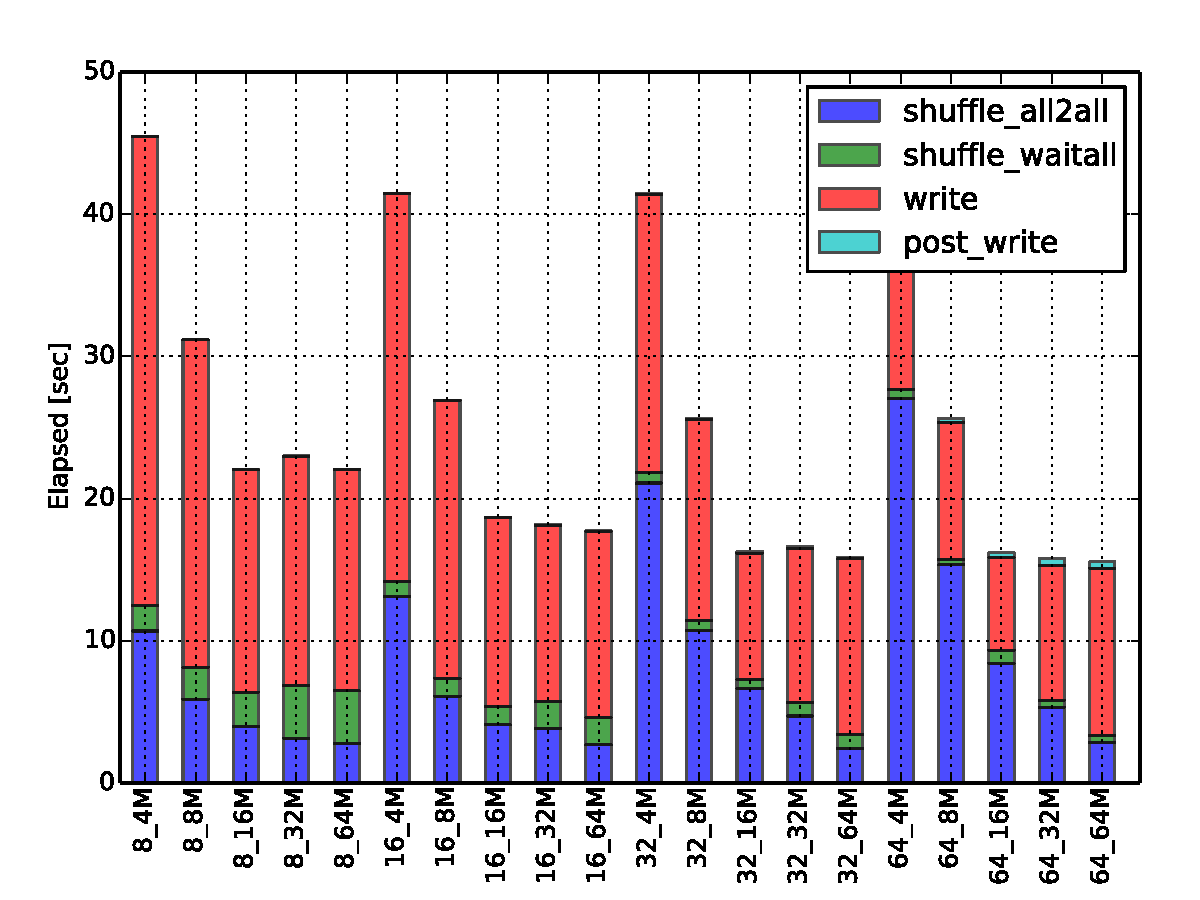
\includegraphics[width=\textwidth]{figures/coll_perf_32GB_30sec_elapsed_disable}
  \caption{}
  \label{figure: collperf-elaps-disable}
  \end{subfigure}
  \begin{subfigure}[]{\textwidth}
  \centering
  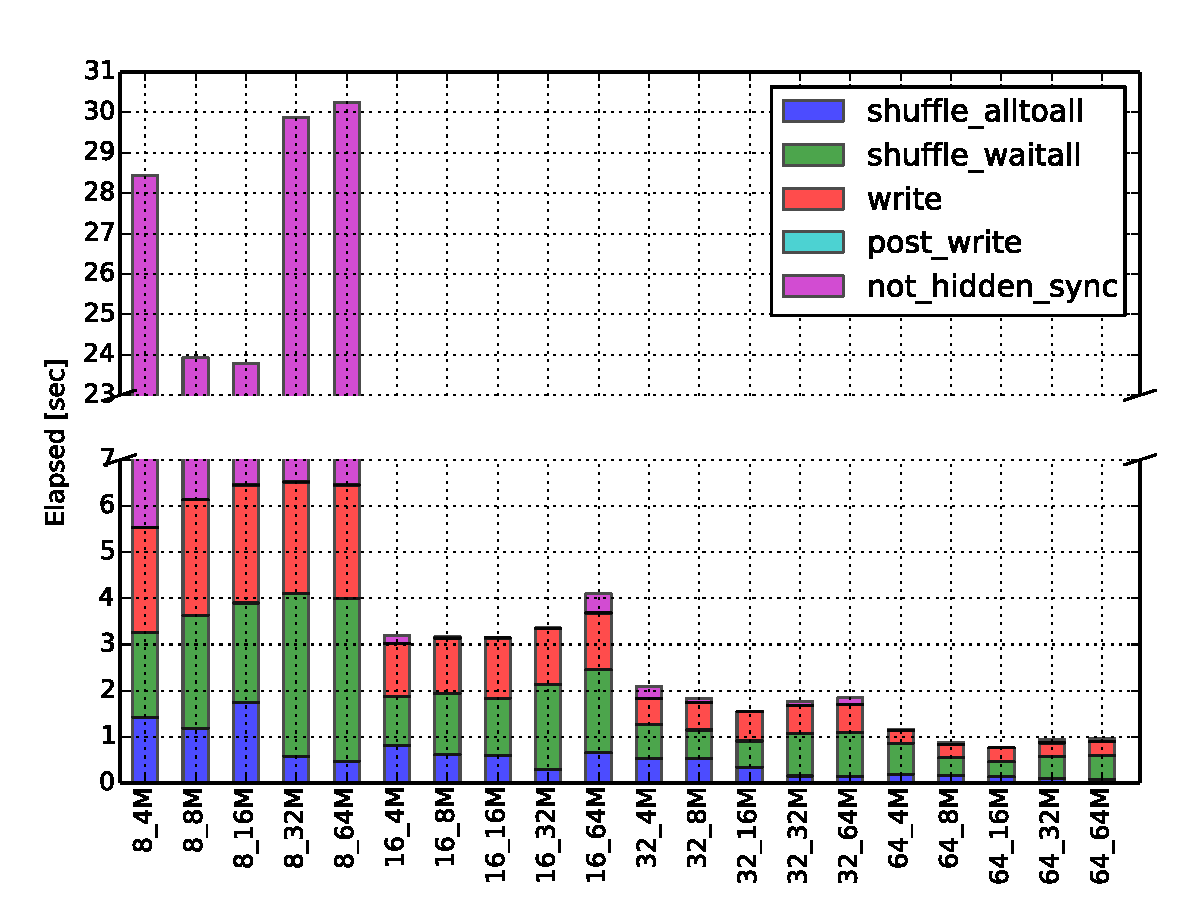
\includegraphics[width=0.7\textwidth]{figures/coll_perf_32GB_30sec_elapsed_enable}
  \caption{}
  \label{figure: collperf-elaps-enable}
  \end{subfigure}
  \caption{Perceived and theoretical write bandwidth for all combinations of aggregators and collective buffer sizes (\ref{figure: collperf-bw}); 
  collective I/O contribution breakdown when cache is disabled (\ref{figure: collperf-elaps-disable}); collective I/O contribution breakdown when cache is 
  enabled (\ref{figure: collperf-elaps-enable}).}
  \label{figure: collperf-results}
\end{figure*}

Figure~\ref{figure: collperf-results} shows the results for the perceived and theoretical write bandwidth (\ref{figure: collperf-bw}), as well as the single 
performance contributions for standard collective I/O (\ref{figure: collperf-elaps-disable}) and cached collective I/O (\ref{figure: collperf-elaps-enable}). 
We start by analyzing the behaviour of standard collective I/O in Figure~\ref{figure: collperf-elaps-disable}.

Let us start by considering the effect of different collective buffer sizes on the collective write time. To this purpose we fix the number of aggregators and look at 
the time contributions when increasing the buffer size from 4~MB to 64~MB. We first observe that the global synchronization cost (\textit{shuffle\_all2all}) decreases.
This is consistent with the ext2ph algorithm behaviour because, as we have already said, increasing the collective buffer size decreases the number of two phase I/O rounds
and therefore the number of global synchronization events (\texttt{MPI\_Alltoall()}). The write cost associated to POSIX write operations also decreases because we are
writing to more I/O servers at the same time (recall that we are using four I/O servers and a stripe size of 4~MB). When the buffer size is 4~MB we only write to one
I/O server, when the buffer size is 16~MB we write to all of them. This also explains why further increasing the buffer size does not reduce the write cost. The
communication cost (\textit{shuffle\_waitall}), on the other hand, increases with the buffer size. This happens because, although the total amount of data shuffled remains
constant, the amount of data shuffled during every round of two phase I/O increases, saturating the aggregators network bandwidth. When we use 8 aggregators, for example, 
up to 32~MB of data are shuffled across the network when using 4~MB buffers, up to 512~MB with 64~MB buffers. Finally, we can look at what happens when we keep the
buffer size constant and increase the number of aggregators. In this case we notice that the global synchronization cost increases. This is due to the increased network 
concurrency at the I/O servers. Finally, \textit{post\_write} time, represented by \texttt{MPI\_Allreduce()}, does not contribute considerably to overall performance because
the corresponding global synchronization event is only encountered once.

We now look at what happens to the ext2ph contributions when we use the cache (Figure~\ref{figure: collperf-elaps-enable}). The global synchronization cost can be still reduced
by increasing the collective buffer size, but because local SSDs are not shared with other nodes across the network, I/O requests can be served in a more predictable way. This
allows aggregators to complete I/O faster and consequently reduces the global synchronization overhead related to collective communications. Write time is not affected visibly
by larger buffers because every aggregator writes data locally. Communication cost is not affected because the communication pattern does not change with respect to the non-cached
collective I/O case. Additionally, we now have a new contribution representing the cache synchronization time that cannot be overlapped with computation (\textit{not\_hidden\_sync}).
We can observe that this contribution is consistent only for 8 aggregators. In fact, when using 8 aggregators the aggregated bandwidth provided by the local SSD
devices cannot match the parallel file system.

The described behaviours are reflected on the perceived write bandwidth shown in Figure~\ref{figure: collperf-bw}. In particular we observe that only the 8 aggregators
configuration achieves worse performance than the standard collective I/O case. All the remaining configurations always achieve better performance and can provide up to
30~GB/s when using 64 aggregators and 32~MB buffer size, an improvement of 15 times. We also observe that the aggregated bandwidth can be scaled by increasing the number 
of aggregators and thus the number of available SSD devices. Finally, when using the cache, the buffer size has limited impact on write bandwidth meaning that we can achieve 
good performance with small buffer sizes, reducing the pressure of collective I/O on system memory.

\subsubsection{Flash-IO}
Flash-IO is the I/O kernel of the Flash application~\cite{Rosner2000}. The Flash-IO benchmark writes three different
files, a checkpoint file a plot file with centered data and a plot file with corner data. The checkpoint file is written using either parallel HDF5 or PnetCDF. We modified the
benchmark to only write the checkpoint file using parallel HDF5. In our configuration, every process in the Flash application writes 80 blocks. Each block contains 16 zones, and 
each zone has 24 variables encoded with 8~bytes, for a total of 768~KBs/block/proc, for a total file size of about 30~GB. Blocks are not written to the checkpoint file with a 
single collective write operation, like in coll\_perf, but instead using multiple collective operations through \texttt{MPI\_File\_write\_at\_all()}. Similarly to coll\_perf we 
have modified the Flash-IO workflow to completely hide the cache synchronization cost.

\begin{figure*}[]
  \centering
  \begin{subfigure}[]{0.7\textwidth}
  \centering
  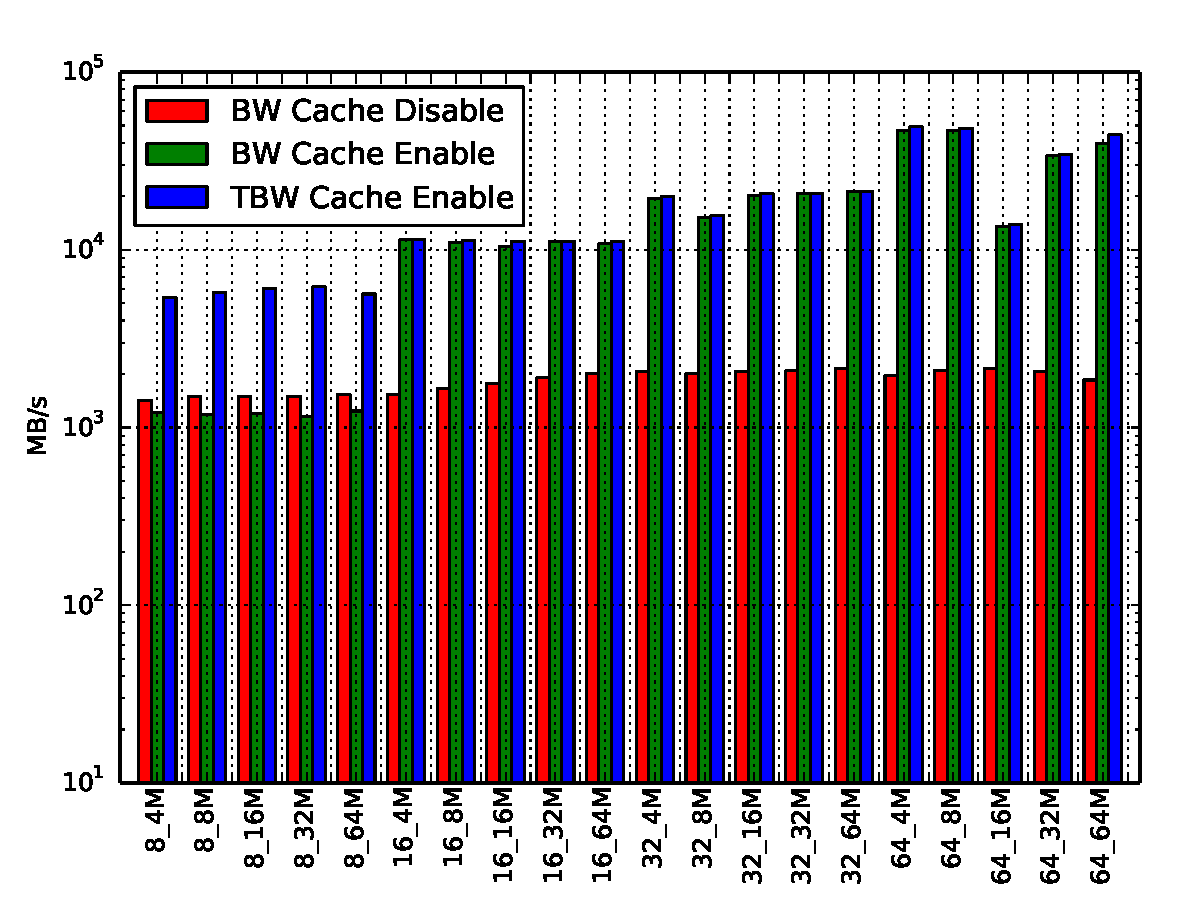
\includegraphics[width=\textwidth]{figures/flash_32GB_30sec_bw}
  \caption{}
  \label{figure: flash-bw}
  \end{subfigure}
  \begin{subfigure}[]{0.7\textwidth}
  \centering
  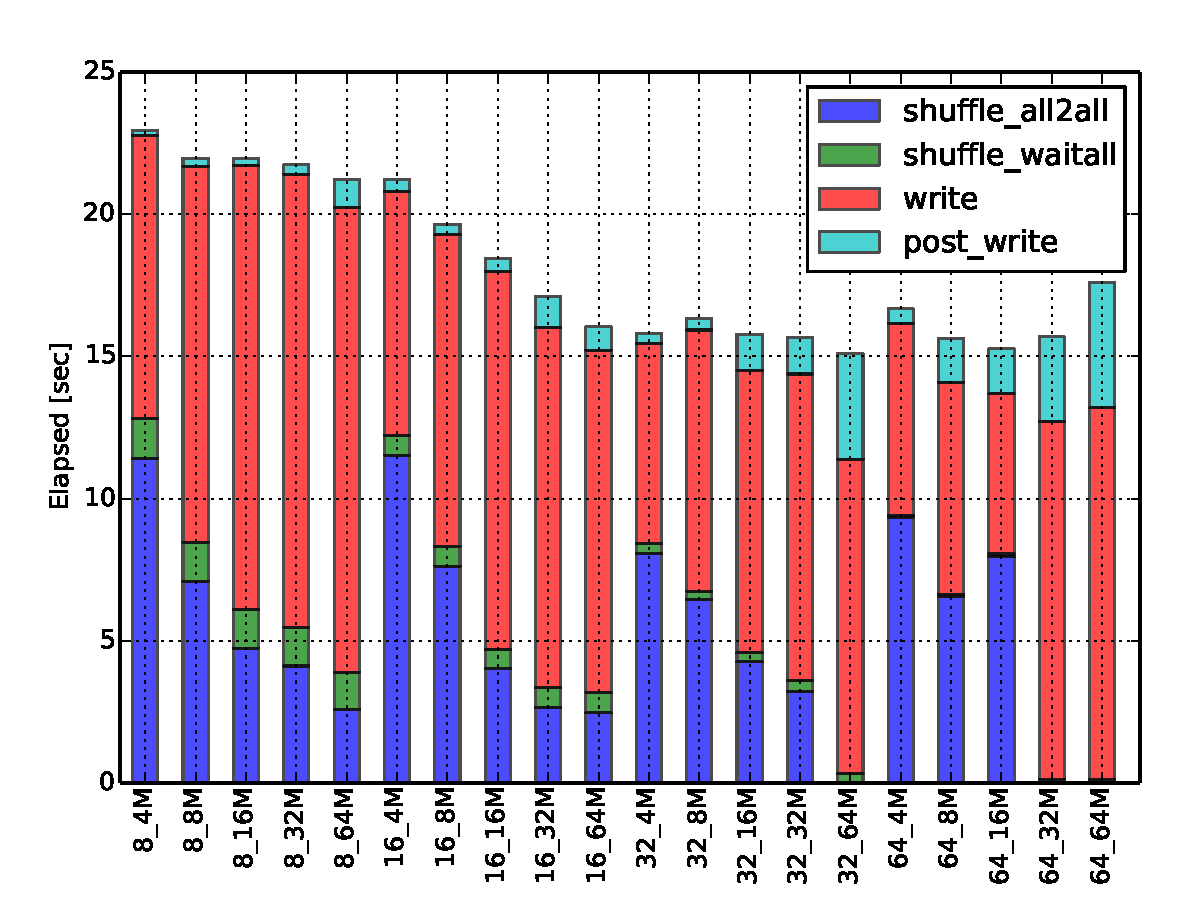
\includegraphics[width=\textwidth]{figures/flash_32GB_30sec_elapsed_disable}
  \caption{}
  \label{figure: flash-elaps-disable}
  \end{subfigure}
  \begin{subfigure}[]{\textwidth}
  \centering
  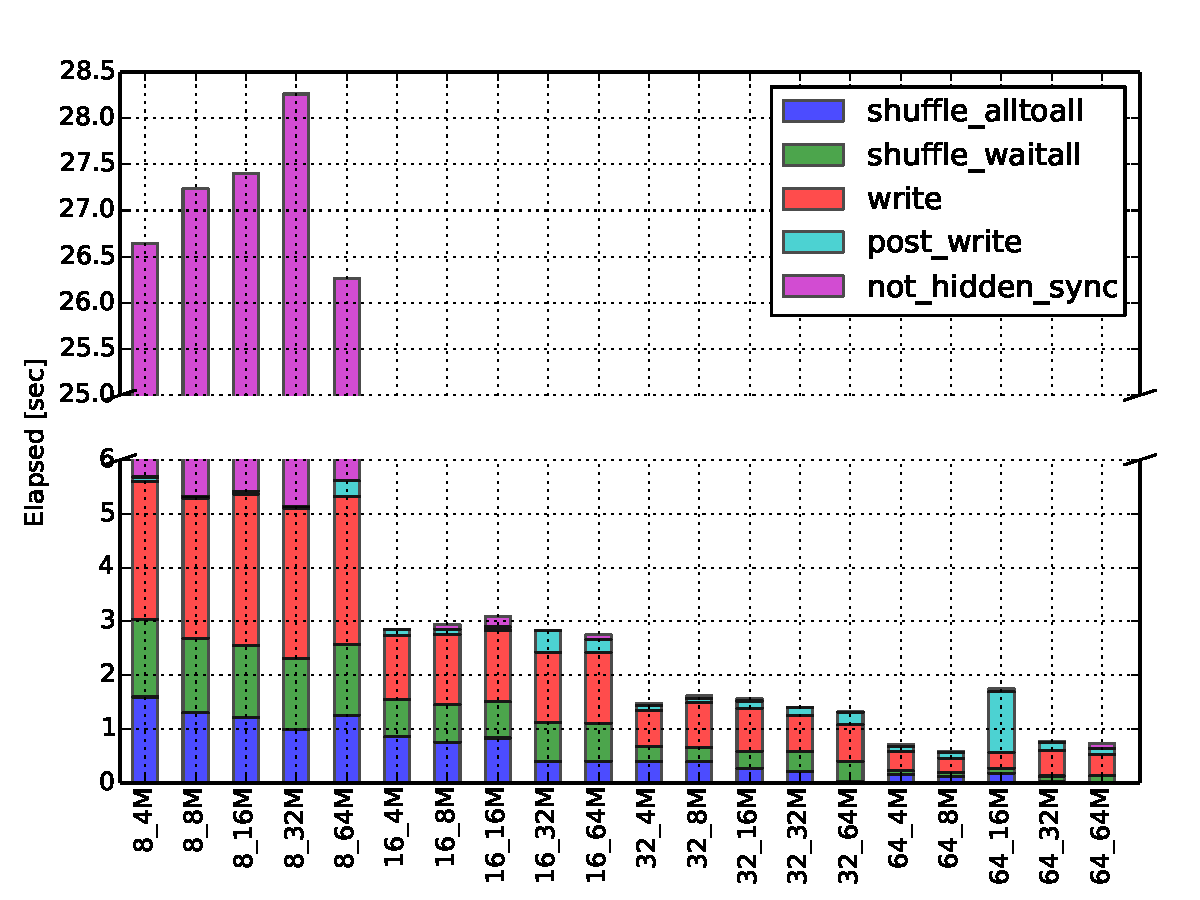
\includegraphics[width=0.7\textwidth]{figures/flash_32GB_30sec_elapsed_enable}
  \caption{}
  \label{figure: flash-elaps-enable}
  \end{subfigure}
  \caption{Perceived I/O bandwidth for all combinations of aggregators and collective buffer sizes (\ref{figure: flash-bw}); collective I/O contribution breakdown 
  when cache is disabled (\ref{figure: flash-elaps-disable}); collective I/O contribution breakdown when cache is enabled (\ref{figure: flash-elaps-enable}).}
  \label{figure: flash-results}
\end{figure*}

Like in coll\_perf, for Flash-IO we measured the same performance parameters varying the number of aggregators and collective buffer size. Results are shown in Figure~\ref{figure:
flash-results}. When the cache is disabled, again we observe reduction of the global synchronization cost for increasing buffer sizes. Communication cost this time does not increase 
with the buffer size. In fact, the file domain size varies from about 49~MB to 6~MB, for 8 and 64 aggregators respectively. This is much less than the amount of data exchanged in 
coll\_perf and thus can be better served by the network infrastructure. Write performance, on the other hand, get worse as the buffer size increases. This behaviour is probably due 
to the fact that, unlike in coll\_perf, writes are not multiple of the stripe size and therefore there might be additional locking overhead at the file system level.
Finally, we observe that the \textit{post\_write} contribution is more consistent this time. The reason, as already anticipated, is that Flash-IO does not write data with a single
collective operation but instead uses multiple operations, thus increasing the number of \texttt{MPI\_Allreduce()} calls at the end of the ext2ph algorithm.

When the cache is enable we can observe much better performance. Once again, 8 aggregators are not sufficient to completely hide cache synchronization cost to the application. As last
note, we see that in the case of 64 aggregators and 16~MB buffer size there is a drop of write bandwidth in Figure~\ref{figure: flash-bw} due to a peak in the \textit{post\_write}
contribution in Figure~\ref{figure: flash-elaps-enable}. This tells us that when using the cache, although we can minimize the scheduling effects on I/O requests, a small variation 
in the I/O time across aggregators can produce substantial effects on the perceived bandwidth. Indeed, we can see a drop of about 25~GB/s with respect to the 64 aggregators and 
32~MB buffer size.

\begin{figure*}[]
  \centering
  \begin{subfigure}[]{0.7\textwidth}
  \centering
  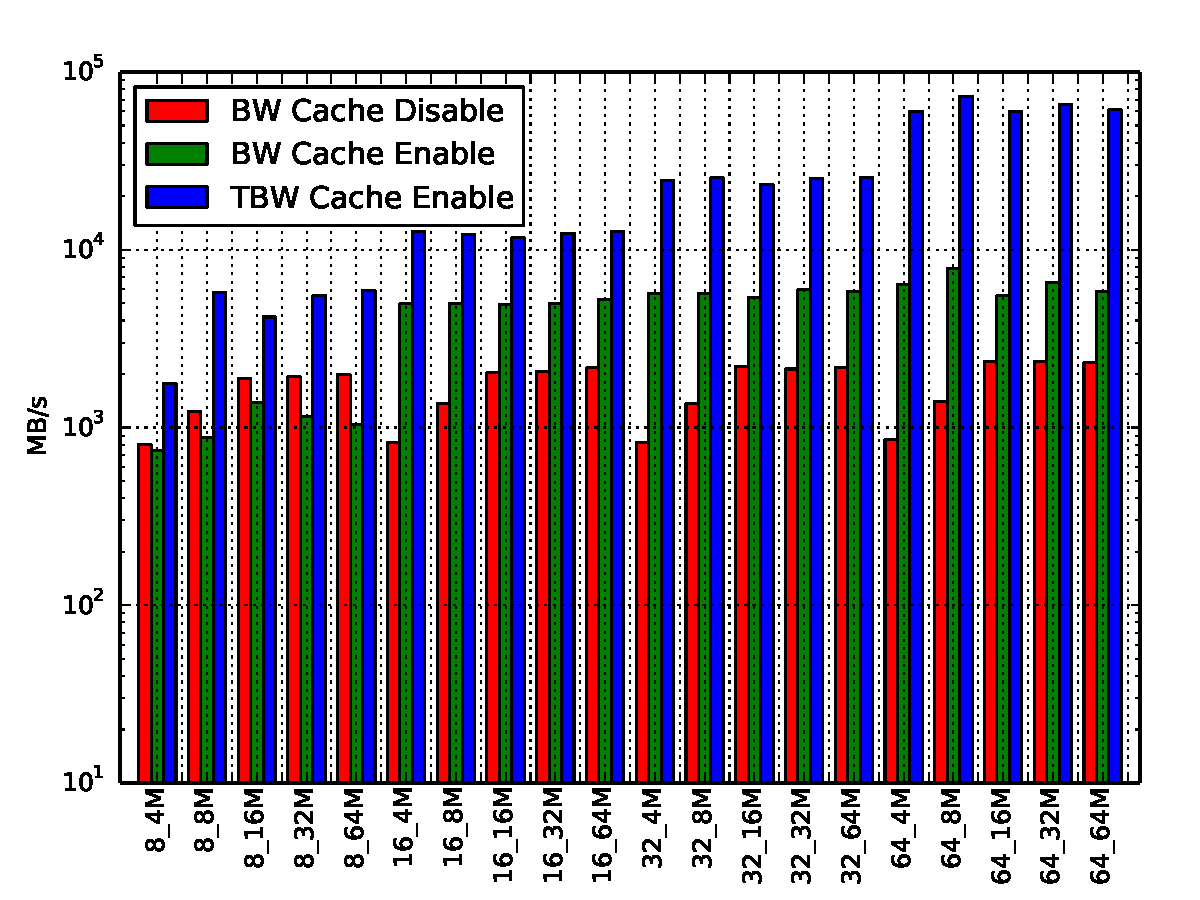
\includegraphics[width=\textwidth]{figures/ior_32GB_30sec_bw}
  \caption{}
  \label{figure: ior-bw}
  \end{subfigure}
  \begin{subfigure}[]{0.7\textwidth}
  \centering
  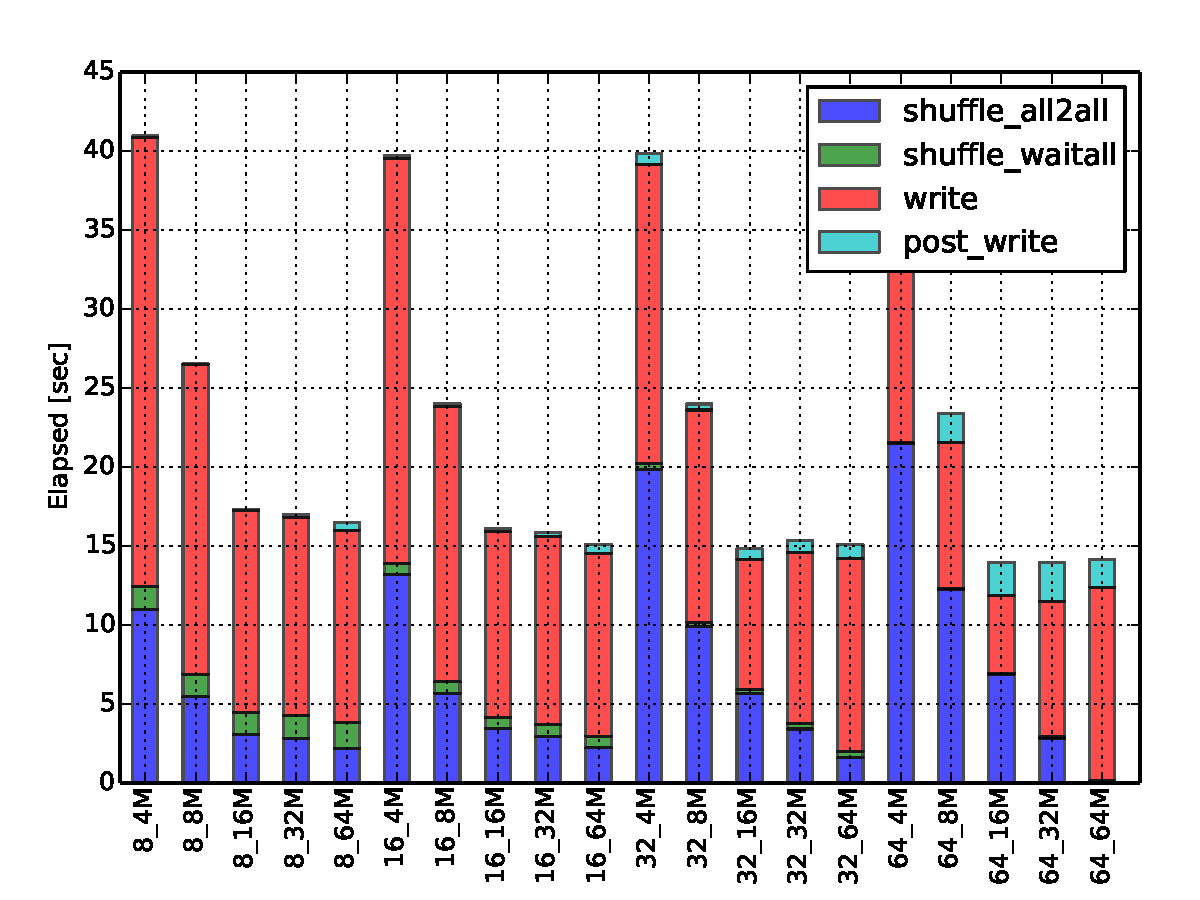
\includegraphics[width=\textwidth]{figures/ior_32GB_30sec_disable}
  \caption{}
  \label{figure: ior-elaps-disable}
  \end{subfigure}
  \begin{subfigure}[]{\textwidth}
  \centering
  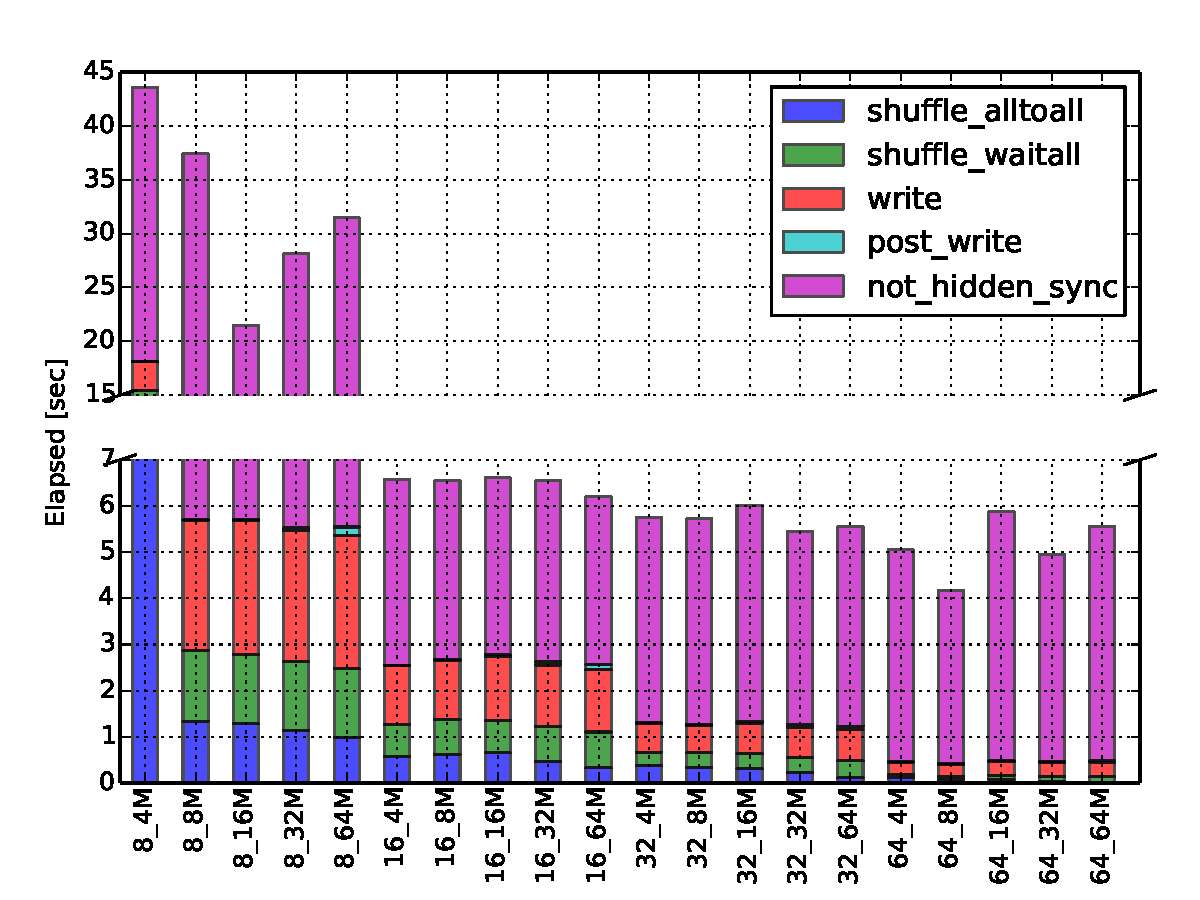
\includegraphics[width=0.7\textwidth]{figures/ior_32GB_30sec_enable}
  \caption{}
  \label{figure: ior-elaps-enable}
  \end{subfigure}
  \caption{Perceived I/O bandwidth for all combinations of aggregators and collective buffer sizes (\ref{figure: ior-bw}); collective I/O contribution breakdown when cache is 
  disabled (\ref{figure: ior-elaps-disable}); collective I/O contribution breakdown when cache is enabled (\ref{figure: ior-elaps-enable}).}
  \label{figure: ior-results}
\end{figure*}

\subsubsection{IOR}
IOR\footnote{\url{http://www.nersc.gov/users/computational-systems/cori/nersc-8-procurement/trinity-nersc-8-rfp/nersc-8-trinity-benchmarks/ior/}.} is a parallel I/O benchmark that supports 
both independent and collective I/O operations using a variety of interfaces including POSIX-IO, MPI-IO and HDF5. Although IOR supports collective I/O operations it does not allow
users to define strided patterns (like the one in coll\_perf) using file views. Strided layouts can be built by reading or writing multiple data segments. A segment is a contiguous byte 
range in the file accessed by only one process. For example, if we have four processes and each of them writes three segments of 64~MB, the first process writes its first segment
starting at 0~MB and ending at 64~MB, the second process writes its first segment starting at 64~MB and ending at 128~MB, and so on.
When all the processes have written the first segment they initiate another write operation for the second segment starting at offset 256~MB. Every segment is written with an independent
collective write operation.

In our experiments we used 8 segments and each of the 512 processes writes 8~MB for segment, for a total of 32~GB file. Unlike the previous two cases, in IOR we follow the workflow
depicted in Figure~\ref{figure: workflow}; meaning that for the last write phase cache synchronization will not be hidden by any following compute phase. This allows us to show what 
a real world use case would look like.

Figure~\ref{figure: ior-results} shows the obtained results. These results are similar to the previous except for the fact that now the \textit{not\_hidden\_sync} contribution is
visible for every collective I/O configuration. The cache synchronization cost represents a huge part of the total I/O time. Although, absolute bandwidth performance are lower 
than previous results we still have that writing data to local SSD devices can give advantages over the baseline ext2ph strategy. In fact, on average we can at least triple the 
perceived write bandwidth going from about 2~GB/s to 6~GB/s.

The reduction of the cache synchronization cost has not been explored in our work and therefore leaves opening for future optimizations that will be discussed in the conclusion
chapter.

\subsection{Conclusions}
In this section we have analyzed collective write performance using a range of different benchmarks that use both synthetic and real I/O patterns to transfer large checkpoint buffers
to the parallel file system. Our tests show how collective I/O is mainly limited by the ext2ph algorithm global synchronization overhead and how the use of fast local non-volatile
memories is effective in reducing the impact that global file system latency has on such synchronization by taking it out of the critical I/O path. Our work practically proves
how next generation I/O systems can benefits from multi tier storage and how first tier non-volatile storage devices can be leveraged by giving the user more control over them.
